% !TeX program = pdflatex
%%=======================================================================
%% GENERATED FILE -- do not edit by hand.
%% Produced by flatten.py from main.tex and sections/*.tex, so that the
%% archive submitted to JMLR contains a single .tex file as its final
%% preparation instructions request.
%% Edit main.tex / sections/*.tex and re-run:  python3 flatten.py
%%=======================================================================
%=======================================================================
% Formal Falsification of the Completeness of a Single Fixed-Memory
% Component for Open Inversion Tasks
%
% LaTeX version in the official JMLR style (jmlr2e.sty, from
% https://github.com/JmlrOrg/jmlr-style-file -- do not modify the .sty).
%
% Environment mapping:
%   LaTeX environment              numbering in the paper
%   ------------------------------ ----------------------
%   claim       (unnumbered)       Claim R
%   uprop       (unnumbered)       Proposition [Mask Criterion]
%   lemma       (shared)           Lemma 1..3
%   proposition (shared)           Proposition 4, 6
%   theorem     (shared)           Theorem 5, 7
%   defn        (separate)         Definition 1..4
%   example     (separate)         Example 1 (the gap-mechanism example of
%                                  Section 5.3; its own counter, so it does not
%                                  disturb the Lemma/Proposition/Theorem chain)
% The lemma/proposition/theorem counter is shared, so the sequence reads
% Lemma 1, Lemma 2, Lemma 3, Proposition 4, Theorem 5 -- exactly as
% referenced throughout the text.
%
% The \acks block required by JMLR (funding and competing-interest
% disclosure) is present below, ahead of the bibliography.
% The \jmlrheading volume/pages/paper-id fields are assigned by the JMLR
% editor at acceptance; they are left empty here.
%=======================================================================

\documentclass[twoside,11pt]{article}

% Any additional packages must be included after jmlr2e.
% jmlr2e already provides epsfig, amssymb, natbib, graphicx and hyperref.
\usepackage{jmlr2e}
\usepackage{amsmath}
\usepackage{array}

% --- theorem environments -------------------------------------------
% jmlr2e defines theorem, lemma, proposition, corollary, remark,
% definition, ... all sharing one counter. The paper numbers definitions
% separately (Definition 1..4), so `defn` gets its own counter; the
% lemma/proposition/theorem counter stays shared, which reproduces the
% numbering Lemma 1, Lemma 2, Lemma 3, Proposition 4, Theorem 5 used in the text.
\newtheorem{defn}{Definition}

% Two unnumbered, named environments (Claim R; Proposition [Mask
% Criterion]). Defined by hand so that amsthm is not needed and the
% official .sty stays untouched.
\makeatletter
\newenvironment{claim}[1][]{\par\medskip\noindent\textbf{Claim\ifx\relax#1\relax\else\ #1\fi:}\ \itshape}{\par\medskip}
\newenvironment{uprop}[1][]{\par\medskip\noindent\textbf{Proposition\ifx\relax#1\relax\else\ (#1)\fi:}\ \itshape}{\par\medskip}
\makeatother

% --- helpers --------------------------------------------------------
% Lead-in of a proof sketch and the right-aligned end-of-proof box,
% reproducing the "Argument." paragraphs of the paper.
\newcommand{\argument}{\par\medskip\noindent\textbf{Argument.}\ }
\newcommand{\qedbox}{\hfill$\square$}
\newcommand{\ev}{\mathrm{ev}}
% Lean declaration names cited in running text are set in \texttt, which does
% not hyphenate, and some of them are a third of the measure long. \ttu is the
% underscore of such a name with a line break allowed after it, so that a
% paragraph citing several names stays free of overfull lines.
\newcommand{\ttu}{\textunderscore\allowbreak}

% --- headline -------------------------------------------------------
% {volume}{year}{pages}{submitted}{published}{paper id}{authors}
% Leave the publication date blank: it is filled in by the editor.
\jmlrheading{}{}{}{9/26}{}{}{Shuo Zhang}
\ShortHeadings{Formal Falsification of Solo Completeness}{Zhang}
\firstpageno{1}

% PDF metadata for the released build (the title/author blocks above are
% typeset by jmlr2e; these fields populate the PDF document properties).
\hypersetup{hidelinks,
  pdftitle={Formal Falsification of the Completeness of a Single Fixed-Memory Component for Open Inversion Tasks},
  pdfauthor={Shuo Zhang},
  pdfsubject={Open inversion tasks; formal falsification; fixed-memory component; decision axis; distributional openness},
  pdfkeywords={open inversion tasks, formal falsification, fixed-memory component, decision axis, distributional openness}}

% --- reproducible output -------------------------------------------
% pdfTeX stamps CreationDate/ModDate from the clock and derives the trailer
% /ID from it, so two builds of identical sources would otherwise differ
% byte-wise. build.sh pins SOURCE_DATE_EPOCH for the dates; seeding the
% trailer id here pins the remaining source of variation. Together they make
% the PDF byte-reproducible, so that a rebuilt paper.pdf differs only when the
% paper's content changed. \ifdefined keeps the file compilable by engines
% without the primitive.
\ifdefined\pdftrailerid
  \pdftrailerid{C0FFEE0123456789ABCDEF0123456789}% synthetic constant, not a real identifier
\fi

\begin{document}

\title{Formal Falsification of the Completeness of a Single Fixed-Memory Component for Open Inversion Tasks}

% NOTE: the author block is present because JMLR submissions are not
% anonymous.
\author{\name Shuo Zhang \email 202400103083@stumail.sztu.edu.cn \\
       \addr Shenzhen Technology University\\
       3002 Lantian Road, Pingshan District\\
       Shenzhen, Guangdong, China 518118}

% The action editor is assigned by JMLR after submission.
\editor{Action Editor}

\maketitle

\begin{abstract}%
Many inference tasks are open inversion tasks, delimited by four criteria: observations are ill-posed, so local observations cannot determine the structure sought; required context strength is heterogeneous and content-addressed by the evidence; inference inputs are unconstrained by the training distribution; and the demand rule cannot be given within any pre-given tolerance by values frozen before inference begins. No fixed-memory component completes such tasks alone; neural networks are its canonical instance. A context rule's content is a set of numbers, from two exclusive and exhaustive sources: current evidence or analytic invariants (Mode A), and corpus statistics or manual setting frozen at inference (Mode B). Generalization on the open set requires Mode A; a fixed-memory component's rules are Mode B. The exclusion holds for any even differentiable pairwise potential, not only the quadratic form: one position whose demand ratio changes between two admissible configurations suffices. What is falsified is solo use, not usefulness. The algebraic skeleton is machine-verified in Lean 4 and Mathlib at general types, with zero sorry and no warnings.
\end{abstract}

\begin{keywords}
  open inversion tasks; formal falsification; fixed-memory component; decision axis; distributional openness
\end{keywords}

%%%%%%%%%%%%%%%%%%%%%%%%%%%%%%%%%%%%%%%%%%%%%%%%%%%%%%%%%%%%%%%%%%%%%%
%% --- inlined from sections/01-introduction.tex
%%%%%%%%%%%%%%%%%%%%%%%%%%%%%%%%%%%%%%%%%%%%%%%%%%%%%%%%%%%%%%%%%%%%%%
\section{Introduction}
\label{ch:intro}

\subsection{Starting from Ill-Posedness}

Many inference tasks are ill-posed: pixel brightness admits infinitely many depths, a measurement infinitely many states, and no local observation alone fixes the answer. In real-time 3D reconstruction, how far is the surface at a pixel? Its color may be weak light from a nearby dark surface or strong light from a distant bright one; under transparency, occlusion, or repetitive texture, still more structures. Observation and structure relate many-to-many---ill-posedness in Hadamard's sense: no solution, no unique solution, or no continuous dependence on the observation \citep{hadamard1902}.

Ill-posedness is intrinsic, not engineering crudeness: observation is structure's residue after projection, sampling, and noise, and no local inverse operation recovers it. Early vision systematized this: stereo, motion estimation, optical flow, and shape reconstruction admit a unique solution only after added constraints \citep{poggio1985}. Those constraints are this paper's context---neighboring pixels on one surface, frames on one motion, voxels in one organ---pinning the degrees of freedom local observations cannot fix.

Context cannot be applied uniformly: strong inside a surface, so the neighborhood corroborates and noise is smoothed away; cut at boundaries and occlusions, so the two sides form independently, else depth smears along edges. Smooth motion lets frames corroborate; abrupt motion demands independence, else the estimate is dragged by history. Strength thus varies with position and time, depending on where the scene's boundaries lie, where motion breaks, and along which contour occlusion occurs---the class's most intractable part: a context rule is not a fixed law but a stipulation varying with the evidence.

\subsection{Open Inversion Tasks}

Four items follow. (P1) Ill-posedness: local observations do not uniquely determine the structure sought, so context is indispensable. (P2) Heterogeneity: required strength varies across positions and instants, and where it should be strong or weak depends on the evidence's content, so boundary locations are content-addressed and cannot be tabulated in advance. (P3) Distributional openness: inference inputs may lie outside the training distribution, the deployment environment's scenes, sensors, and motion patterns unbounded by the training corpus---the \emph{open set}. (P4) Non-freezable demand: the context rule, as a mapping from evidence to strengths, cannot be given within any pre-given tolerance on the open set by values frozen before inference begins. A task satisfying all four is an \emph{open inversion task}.

Real-time 3D reconstruction is typical: pixelwise ill-posed depth, heterogeneous smoothing inside and outside boundaries, environments unconstrained by the training set; recent real-time radiance-field reconstruction \citep{kerbl2023} pushed this form to the engineering foreground. Image and video restoration: mixed degradation kernels and noise levels make local observations ill-posed, textured and flat regions demand different restoration strengths, and real degradations exceed synthetic training sets. Online state estimation: the measurement equation is ill-posed along weakly observable directions, process-noise strength switches with the motion mode, and the open world supplies out-of-distribution operating conditions. Medical and scientific inversion, from tomographic reconstruction to inverse scattering, also falls within this framework.

These four items are premises, not conclusions, for large classes of real tasks: inverse problems mostly ill-posed, the defining feature of Hadamard's criterion; natural data mostly heterogeneous, boundaries, occlusions, and abrupt changes being natural signals' structure rather than exceptions; online systems mostly open, and removing train--test distribution agreement voids the guarantees statistical learning theory built on it \citep{vapnik1995}. But not universally: homogeneous interpolation fails heterogeneity, the required smoothing strength uniform; fixed-grid numerical simulation sets boundary positions by the task, not evidence content; fixed operating conditions prescribe the strength demand by an exogenous schedule. These three families are not open inversion tasks, and fixed-memory components on them lie outside what this paper falsifies. The fourth boundary: if the demand is exactly identifiable from a fixed corpus---e.g.\ a linear function of the evidence pinned by a few noiseless samples---a frozen component can be complete, so such tasks are not open inversion tasks, falsification stopping exactly where the demand becomes freezable. By Section~\ref{sec:p4}, such a task fails the barrier condition: its demand has a pre-given modulus, no separation surviving at fine scale.

\subsection{The Claim to Be Falsified}

Since context rules are this class's core: is there a component that, by itself alone, applies them correctly on every open inversion task? This is no straw man but the conjunction of two public claims. First, the engineering corollary of universal approximation theorems \citep{cybenko1989,hornik1989}: neural networks approximate arbitrary functions and inference maps observations to structures, so a large enough network with a large enough corpus should in principle suffice---the implicit premise of systems work on end-to-end 3D reconstruction and online estimation. Second, the scale claim \citep{bubeck2023}: contextual deficiencies are a matter of corpus and parameter scale, not architectural category, its critics noting some so-called emergent abilities may be artifacts of metric choice \citep{schaeffer2023}. Together they assert some fixed-memory component, once at scale, completes the task on its own---exactly what this paper falsifies:

\begin{claim}[$\mathcal{R}$]
There exists a fixed-memory component that, using only that component and without any external proposal or arbitration stage, is complete for open inversion tasks; that is, it completes the task independently in the sense of the open set, of no distribution agreement, and of cross-scenario reuse.
\end{claim}

A fixed-memory component freezes its context rules into parameters fixed at inference time, valued from training-corpus statistics or manual setting; its literature counterpart is parametric amortized inference's carrier, a forward process with fixed corpus-determined parameters. Mode A does not exclude parameters---analytic invariants are parameters too---the difference being the source: calibration and geometry, not corpus statistics. Completeness here is independent completion in task capability, not logical completeness of formal systems. Neural networks are the canonical instance, the context rule carried in training- or calibration-derived weights; Theorem 5 instantiates Claim $\mathcal{R}$ on this carrier, the neural-network-only claim $\mathcal{P}$.

The qualifier ``only'' is crucial: what is falsified is solo use, not these components' usefulness within combinations---neural networks as feature extractors can serve in larger systems. High accuracy on a fixed benchmark close to the training distribution is within reach of both kinds of networks, but that \emph{weak claim} is not the object here: whether the component alone, as a general-purpose inference mechanism, completes tasks independently, possessing completeness in the task sense. The weak claim's truth and the strong claim's falsity are compatible, as an instrument extremely accurate under standard operating conditions may still fail to work independently under arbitrary ones.

\subsection{Method of Falsification and Structure of the Paper}

Method is deduction, not experiment: Claim $\mathcal{R}$ is existential and its negation universal over a whole task class, so no single counterexample refutes it Popper-style \citep{popper1959}---refutation needs a deductive chain from the class's defining criteria (which must first pin the class down) to the component's capability boundary. All derivations are formal, with no experimental data: experiments exhibit symptoms, but what this paper proves is the crux. The algebraic core is independent of the classical variational problem's quadratic smoothing form; Lemma 1 holds for a separable data term, arbitrary even differentiable pairwise potential, no convexity, so it covers nonconvex objectives' stationary points too. It excludes the frozen coefficient family in general---the global scalar its shallowest case---with the minimal obstruction an equivalence, not a sufficient condition: one position whose required strength ratio changes between two admissible configurations excludes every frozen family, however many entries. Whether the criteria capture real tasks is empirical; the paper discusses when each holds, and what lies outside them is a class boundary, not a counterexample. \emph{Falsification} is deductive: Claim $\mathcal{R}$ is refuted under Criteria P1 to P4, and Section~\ref{ch:verify} delimits the term where machine verification is described.

%%%%%%%%%%%%%%%%%%%%%%%%%%%%%%%%%%%%%%%%%%%%%%%%%%%%%%%%%%%%%%%%%%%%%%
%% --- inlined from sections/02-related-work.tex
%%%%%%%%%%%%%%%%%%%%%%%%%%%%%%%%%%%%%%%%%%%%%%%%%%%%%%%%%%%%%%%%%%%%%%
\section{Related Work}
\label{ch:related}

Amortization replaces per-instance optimization by a corpus-fixed recognition network---the inference-theoretic form of Mode B, continued by simulation-based and amortized-inference workflows \citep{cranmer2020,radev2023}---and its amortization gap to the per-instance optimum, an attributable component of VAE-type suboptimality \citep{cremer2018}, is isomorphic to Lemma 3's risk gap (Mode B fixed function family to amortized family, Mode A instantiated rules to the per-instance optimum), evidencing beyond the toy instance that the gap is positive. Operators keeping it open---loopy belief propagation, structured variational inference, learned proposals---change cost and accuracy, not provenance (Section~\ref{ch:falsify}). The sharpest Mode~B instances are the diffusion-prior reconstructors DAVI, a measurement-to-posterior-distribution map, and U-DAVI, with uncertainty-guided training: frozen maps replacing per-instance optimization \citep{lee2024davi,varshney2026udavi} whose strength on unseen measurements is exactly the weak claim bounded here. The semi-amortized family refines an amortized initialization per instance by stochastic variational inference \citep{kim2018semi}---Mode~B initialization plus Mode~A refinement, not a third mode.

Per-instance optimization---each input solved separately with rule values instantiated by current evidence---is Mode A, as is transduction, which exploits test points at inference time \citep{vapnik1995} but assumes test and training distributions agree, whereas the open-set case is stronger; it precedents Mode A under near-distribution conditions, and the novelty here is Mode A as a necessary condition for open inversion, not an optional strategy.

The No-Free-Lunch family is the closest relative to this paper. The original form averages performance uniformly over \emph{all} problems and concludes that no algorithm dominates universally \citep{wolpert1996}; its premise, the uniform average, flattens task structure and says nothing about completeness on a task class. The companion result gives the other half: with an explicit prior or assumption, a priori distinctions between algorithms \emph{do} exist \citep{wolpert1996b}, a later retrospective locating the point of NFL in the premises rather than the slogan \citep{wolpert2021}. The optimization version moves the conclusion into search \citep{wolpert1997}; the conservation-of-performance reading rewrites ``indistinguishability under uniform averaging'' as ``improving one class must be paid for by degradation on another'' \citep{ho2002}. Statistical learning theory gives the hypothesis-class version: learning is impossible on unrestricted classes without inductive bias and PAC learnability requires controlled capacity \citep{shalev2014}, while an explicit task distribution lets the bias be learned across tasks \citep{baxter2000}; the decidability of some learning problems is itself undecidable \citep{bentdavid2019}. Conceptual work states which conclusion depends on which notion of uniformity \citep{sterkenburg2021}, reviewed in \citet{adam2019}.

This paper instantiates Wolpert's converse on open inversion tasks; see Table~\ref{tab:nfl}.

\begin{table}[t]
\caption{This paper compared with the No-Free-Lunch family}
\label{tab:nfl}
\centering
\small
\begin{tabular}{@{}>{\raggedright\arraybackslash}p{0.15\textwidth}>{\raggedright\arraybackslash}p{0.24\textwidth}>{\raggedright\arraybackslash}p{0.24\textwidth}>{\raggedright\arraybackslash}p{0.25\textwidth}@{}}
\hline
\textbf{Dimension} & \textbf{No-Free-Lunch family} & \textbf{Bias necessity in statistical learning} & \textbf{This paper}\\
\hline
Object of negation & Algorithms under uniform averaging over all problems & Learners without inductive bias & Fixed-memory components, namely rule carriers of frozen provenance\\
\hline
Level of negation & Algorithm level & Hypothesis-class level & Component level\\
\hline
Load-bearing premise & A uniform measure over problems & Unlimited capacity of the hypothesis class & Criterion P4, non-freezability of the demand\\
\hline
Average or pointwise & Averaged over all problems & Uniform convergence in-distribution & Uniform pointwise bound inside the task class\\
\hline
Relation to task structure & Flattens task structure & Requires a prior or capacity control & Fixes the task structure P1 to P4\\
\hline
Testability of the premise & The uniform measure is untestable & Capacity is estimable & P4 admits a testable statement\\
\hline
Consequence of the negation & No algorithm dominates universally & No learning without bias & Frozen provenance cannot carry the guarantee; Mode A is the only route left\\
\hline
\end{tabular}
\end{table}

Three remarks. First, this paper is the converse of NFL, not a contradiction: NFL denies a distinction without a prior, whereas given P1 to P4 and the value-source dichotomy the distinction exists and falls on the side of the modes. Second, the levels differ: NFL and capacity theory act at algorithm or hypothesis-class level, this negation at component level---inside one task class no carrier whose rules are borne by frozen values satisfies a uniform bound---independently of whether any algorithm class is globally optimal. Third, the premise differs: NFL's uniform measure is untestable in real settings, whereas P4 is testable with two separately addressable components, the barrier condition by demand comparison across scales and the realization level by the frequency of fine-scale demand reversals (Section~\ref{sec:p4}); the theorems here thus have exactly the force of P4, a sufficient condition implying a bound rather than restating it (Section~\ref{ch:falsify}).

One possible objection: given assumptions a distinction exists, so is the specialization trivial? Its significance lies in the manner and products, not the existence. First, the conclusion's form changes: NFL's converse yields a comparative ordering in the average sense, this paper a pointwise impossibility inside a task class: a step from degree to kind. Second, the invariant distinguished is invisible to NFL, which sees behavior but not the value source; here the distinction falls on the source, so behaviorally identical systems land on opposite sides. Third, NFL's prior is arbitrary whereas the criterion here is testable, so the theorem can be challenged empirically, while an untestable uniform measure yields no cumulative conclusion. Fourth, the conclusion's shape differs: an ordering answers which algorithm to swap, a boundary which class of architecture, and the boundary here yields design implications and a cost trade-off. Fifth, the premise is pinned in the open, making stronger evidence for P4, an adjusted task class and A0 upgraded to certifiability cumulative future work; the machine-verified algebraic skeleton further turns an existence argument into an auditable object.

Distributional robustness and invariance in the training objective responds to the open set by changing what is optimized, not where inference-time values come from: distributionally robust optimization minimizes a worst case over an ambiguity set around the corpus \citep{bental2013,rahimian2022}; invariant risk minimization seeks a representation whose optimal predictor is simultaneously optimal across training environments, so the invariant part should transfer \citep{arjovsky2019}; group-robust objectives minimize the worst group risk given group labels, stressing the regularization such minima need \citep{sagawa2020}; domain generalization trains on several source domains to transfer to an unseen one \citep{zhou2022}, controlled benchmarks reporting a tuned empirical-risk baseline a strong competitor \citep{gulrajani2021}. Part of this branch also adapts at test time, classified by the provenance of its update rule (sixth branch).

The axis classifies this branch rather than competing: every intervention acts on the training objective or fitted representation, none on the source of the numbers carrying the inference-time rule, since all these objects are corpus-given and the predictor's parameters are fixed at inference time, hence Mode B however selected. Not a defect but the consequence of the question each answers: how to select among frozen values for better behavior on uncovered inputs, whereas the axis asks whether frozen values can carry the guarantee. A robust objective can thus improve the weak claim, where the literatures agree, but not the positive claim, which Criterion P4 excludes. A DRO worst case is defined by an ambiguity set fixed before inference, the open set here by no set; whether that set contains the deployment condition is an assumption of the same family as training-test agreement, failing likewise when the corpus does not span the operating conditions. Two boundaries: invariance is a property of a frozen representation, so invariant-feature learning shifts the burden from predictor to representation, not the value source; robustness is purchased against a preset set, so its guarantee is inherited from the ambiguity set, not generated from current evidence---the distinction the axis draws.

Hypernetworks generate one network's weights with another \citep{ha2016}. The generator is the counterpart of the ``move one level up'' mechanism of the reach section: its generated weights are inference-time values, but its own values are corpus-given frozen parameters, so Mode B moves up one level and the ultimate source remains the corpus. The generator is itself a rule: corpus-fitted, Mode B; analytic---weights computed by projective geometry---Mode A by the implementer clause of Definition~3, as the procedure of Section~\ref{sec:procedure} asks of any rule. Recursion adds no value source, only provenance length.

Meta-learning and online adaptation change values at inference time, so whether they leave the fixed-memory class is the boundary case the axis settles. Meta-learning fits, across a task distribution, an initialization or update rule giving an adapted predictor after a few steps \citep{finn2017}, surveyed by \citet{hospedales2021}; test-time adaptation updates parameters from the test input, typically self-supervised \citep{sun2020}, now a methodological spectrum \citep{liang2024}. Both are classified by the provenance of the update rule, not its occurrence: a corpus-fitted rule, frozen at the new task, carries adaptation by a corpus-borne rule---Mode B moved up one level---whereas a rule in closed form from the current evidence, as a Kalman gain or a strength solved by Stein's unbiased risk estimation, instantiates its values in the evidence and is Mode A. Few-shot meta-learned adaptation and a single per-instance optimization step both update parameters at test time yet land on opposite sides (Section~\ref{sec:procedure}), so leaving the fixed-memory class is not escaping the negation: what escapes is the limit instantiated by current evidence, not that an optimizer ran, and steps from a corpus-initialized point, or a learned initialization, have not moved the value source. The control-theoretic and online-learning counterparts---gain scheduling, auto-tuning and model-reference adaptive control, and updates along the current loss sequence---recompute the rule each step and are Mode A by source \citep{shamma1990,astrom1995,hazan2016}, their guarantees and gap to the present setting discussed in Section~\ref{ch:discussion}.

Classical regularization's parameter-selection tradition has known the limitation of fixed strength since Tikhonov \citep{tikhonov1977}, developing the L-curve \citep{hansen1992} and generalized cross-validation \citep{golub1979}; Lemma 1 algebraizes it into a contradiction at the level of optimality conditions and notes that offline selection still yields a frozen table, hence Mode B. Its Mode A precedents---Stein's unbiased risk estimation from the current noisy observation \citep{stein1981}, anisotropic diffusion and the guided filter taking position-wise weights as fixed functions of the current evidence computed online \citep{perona1990,he2013}, empirical Bayes estimating prior hyperparameters from the current data---share the extrinsic form of Paradigm E while their source is Mode A: the form is not the criterion (Section~\ref{ch:falsify}). Hybrid inverse methods combine the two: plug-and-play priors let a denoiser carry the prior while an analytic data-consistency step produces the solution \citep{venkatakrishnan2013}, and regularization by denoising writes a denoiser's prior into an explicit regularizer \citep{romano2017}; both decompose credit as the reach section requires, a frozen prior contributing a Mode B candidate without guarantee and an evidence-evaluated data-consistency step the analytic criterion. Data-consistent learned reconstruction combines a frozen prior with analytic measurement consistency \citep{haltmeier2026}, frozen components proposing candidates with analytic constraints carrying the guarantee, and performs robustly within and somewhat beyond the training distribution on a standard benchmark \citep{leuschner2021}---a weak-claim success consistent with the delimitation here and detailed in the composite-path section of Section~\ref{ch:discussion}.

The mathematical theory of memory grounds deep representation learning as learning structured representations of low-dimensional distributions from data, calling such a representation empirical memory \citep{buchanan2026}, with white-box networks interpreting frozen weights as unrolled optimization algorithms; it closes by stating that open-ended models, however large, belong to a closed world, that open worlds require closed-loop systems with online error correction, and that regeneration from memory is only the lowest level of its hierarchy of intelligence. The increment here is to turn that position into a decidable deductive chain with Criteria P1 to P4 whose algebraic skeleton is machine-verified.

%%%%%%%%%%%%%%%%%%%%%%%%%%%%%%%%%%%%%%%%%%%%%%%%%%%%%%%%%%%%%%%%%%%%%%
%% --- inlined from sections/03-formalization.tex
%%%%%%%%%%%%%%%%%%%%%%%%%%%%%%%%%%%%%%%%%%%%%%%%%%%%%%%%%%%%%%%%%%%%%%
\section{Formalization of the Problem}
\label{ch:formalize}

\subsection{Observations, Structure Fields, and Ill-Posedness}

The position set $I$ is the pixel set for image tasks, and the product of time indices and state components for state estimation; the structure field $d : I \to \mathbb{R}$ assigns each position a structure value---depth, intensity, a state component. An observation is a mask $m : I \to \{0, 1\}$ plus the observed masked values; values inside the mask are pinned, those outside unconstrained.

\begin{defn}
An observation is \emph{ill-posed} if two different structure fields $d \neq e$ agree with the observed values at every position inside the mask.
\end{defn}

\begin{uprop}[Mask Criterion]
An observation with a hole is ill-posed: if some position $j$ is not covered by the mask, two different values at $j$ give two structure fields compatible with the same observation. Conversely, a full mask determines the structure field uniquely, so the observation is not ill-posed.
\end{uprop}

Neither direction depends on numerical detail: unmasked positions are degrees of freedom, two values on one giving a bifurcation; a full mask pins every position. Real observations almost always have holes: depth behind occluders, bands drowned in noise, null spaces of measurement equations.

\subsection{Four Criteria}

\begin{itemize}
\item Criterion P1 (ill-posedness): The observation is ill-posed---different structure fields fit the same observation.
\item Criterion P2 (heterogeneity): The required context strength is non-constant: boundary and interior positions need different consistency strengths, and which are boundary is fixed by the current evidence.
\item Criterion P3 (distributional openness): Inference inputs are not constrained by the training distribution; its decidable form, \emph{mask openness}, pins the evidence part by the observation while the context part retains uncovered free positions, so the same evidence admits free bifurcation of the context values.
\item Criterion P4 (non-freezability of the demand): The demand rule's values---the task's target profile at each position---cannot be given within any pre-given tolerance on the open set by any object existing before inference begins. Section~\ref{sec:p4} splits it into a \emph{barrier condition}, that the demand separates nearby instances by a fixed amount at every scale, hence has no pre-given modulus, and a \emph{realization condition}, that the separated instances carry probability bounded away from zero under the test distribution; together they imply a positive floor $\kappa$ on the risk gap of any offline-frozen rule versus the optimal evidence-instantiated risk, Section~\ref{ch:falsify} consuming the instance at the tolerance under discussion.
\end{itemize}

P3 implies P1, mask openness being a hole. Open inversion difficulty is thus a progression layer upon layer, not a sum: ill-posedness forces context use, heterogeneity makes context position-dependent, openness demands correctness on unseen inputs, non-freezability demands an unpinnable offline demand. Section~\ref{ch:falsify} consumes the four criteria in turn.

\paragraph{Two terms, one notion.} \emph{Distributional openness} names the property: inference inputs are not constrained by the training distribution, so the corpus bounds no region where a rule could be certified. \emph{Mask openness} is its decidable form: the evidence part pinned by the observation, the context part retaining uncovered free positions, so the same evidence admits free bifurcation. The two are related by a claim, not a definition---mask openness is the decidable content, not a model of distribution shift---and it alone the derivations of Section~\ref{ch:falsify} consume. \emph{The open set} means the inputs admitted by Criterion P3, not a topological term; ``on the open set'' never means the mask condition. The test distribution's measure is unspecified; Lemma 3 in Section~\ref{ch:falsify} holds for any probability measure.

P4 alone is not readable off the task syntax: like the other three, no definitional clause, its satisfaction depending on task structure. The linear-demand example of Section~\ref{ch:intro} marks the boundary: a pinnable demand lets a fixed-memory component be complete, so the task leaves the class. The positive claims need one further feasibility assumption, separate from the criteria, entering only with Mode A.

\paragraph{Why P4 is not definitional.} Three properties answer the objection that P4 presupposes the conclusion. First, the class is defined by P1 to P3, yet the linear-demand task of Section~\ref{ch:intro} satisfies all three with a demand pinned down by fixed numbers, so a frozen component is complete and P4 fails: failure of P4 is substantive, not definitional, a class admitting such members not being defined by the negated claim's failure. Second, the barrier condition of P4a mentions no rule, average, or benchmark---only the demand's dispersion, in the family of classical approximation barriers \citep{kolmogorov1936,pinkus1985}---and is falsifiable across scales, since a demand Lipschitz in the instance with a modest constant fails it. Third, the transmission from the two components to a risk gap is an inequality proved in Section~\ref{sec:p4}, not assumed, so empirical content sits in the realization level $p$ and the benchmark risk of the best evidence-instantiated rule. The claim that the theorems' force equals P4's is retained in Section~\ref{ch:falsify}, sharpened: P4 suffices to imply a bound, not restate it.

\begin{itemize}
\item Assumption A0 (evidence-computability of the demand): The demand rule is computable from current evidence: a mapping from evidence to the demand rule's values such that on every input the demanded values can be given at inference time by evidence and analytic means.
\end{itemize}

A0 plays no role in the negation of Mode B, which consumes only P1 to P4; it supports the positive reading of Section~\ref{ch:discussion}. On typical tasks the boundaries where context must be cut are visible in the evidence, so the occluded thing is the structure, not the rule; tasks whose demand depends on unobserved structure and leaves no evidence trace do not satisfy A0, remaining within the falsification but outside the positive claims.

Representation of the structure field is unrestricted: depth may be a scalar field, disparity, a signed distance field, or multivectors of geometric algebra \citep{hestenes1984,dorst2007}, and the mask form and four criteria hold under all, ill-posedness and heterogeneity being properties of observations and tasks. Subsequent arguments cite only the mask form of the observation and the source of the context values, hence are representation-independent.

%%%%%%%%%%%%%%%%%%%%%%%%%%%%%%%%%%%%%%%%%%%%%%%%%%%%%%%%%%%%%%%%%%%%%%
%% --- inlined from sections/04-decision-axis.tex
%%%%%%%%%%%%%%%%%%%%%%%%%%%%%%%%%%%%%%%%%%%%%%%%%%%%%%%%%%%%%%%%%%%%%%
\section{The Decision Axis: Context Rules and Two Modes}
\label{ch:axis}

\subsection{Context Rules}

Ill-posed tasks cannot do without context (Section~\ref{ch:formalize}), but ``using context'' needs an analyzable handle:

\begin{defn}
A \emph{context rule} stipulates where and how strongly context is needed, its content being a set of numbers: a family $R = (R_i)_{i \in I}$ of mappings $R_i : (I \to \mathbb{R}) \to \mathbb{R}$, where $R_i$, given the current evidence and a candidate structure field, yields the strength with which context is to be used at position $i$. It is \emph{global} when the family is constant, $R_i = R_j$ for all positions $i, j$, as in the scalar $\lambda$ of classical regularization, and \emph{position-wise} when not, so that the strength used can differ by position.
\end{defn}

Describing a rule as numbers is no simplification: symbolic constraints or program fragments must still be instantiated numerically to enter numerical inference, so representation changes the rule's carrier, not the classification of the source of its values; whatever face a rule wears --- a regularization coefficient, a network's implicit preference --- it enters inference as numbers, so the correctness problem of the rule becomes the source problem of the numbers.

The index carries content: criterion P2 requires the context strength to differ across positions, the evidence content-addressing which are boundary and which interior, so a rule that cannot vary by position cannot express the demand it must meet. Whether a constant family can nonetheless meet it, Lemma 1 of Section~\ref{ch:falsify} answers in the negative, and the position-wise family is the form of the Mode A constructions of the reach section.

\subsection{Mode A and Mode B}

\begin{defn}
A rule is \emph{Mode A} if all its values are instantiated by current evidence or taken from cross-scenario invariants given by analysis and calibration, such as camera intrinsics; it is \emph{Mode B} if its computation involves parameters fixed at inference time whose values come from training-corpus statistics or manual setting. The two are mutually exclusive and exhaustive. Only parameters carrying the rule's content --- those whose variation changes its values --- participate: per-instance optimization contains solver values fixed at inference time that affect the speed of approaching the limit but not the limit itself, so classification follows the limit, which evidence instantiates, and such implementations remain Mode A. What is classified is the source of the function, not its carrier: a component implementing an analytic or calibration function with fixed parameters is Mode A, its values' substantive source being an analytic invariant; one implementing a corpus-statistical function remains Mode B even if what it computes depends only on evidence.
\end{defn}

The functional-dependence view bases inference on the function computed, this axis on the source of the values; the two agree except in the two boundary situations named above. The axis answers who carries the correctness guarantee, the functional-dependence view what the behavior is. Behavioral out-of-distribution robustness, often achieved in practice, is a weak claim compatible with the negation of this paper. Hypernetworks and test-time adaptation are classified by Section~\ref{sec:procedure} and the reach section of Section~\ref{ch:falsify}.

Mutual exclusivity and exhaustiveness: a number either comes into existence at inference time, from the current input or by geometric calibration, or pre-exists inference in some parameter slot; there is no third state. Training-corpus statistics and manual setting belong to the latter, differing only in the production process, not the time of existence: a 0.37 distilled from corpus statistics and a 0.37 written down by an engineer are both pre-existing fixed numbers at inference. Cross-scenario invariants are Mode A because analysis and calibration carry no corpus-specific statistical memory: camera intrinsics are fixed by projective geometry for this frame and every other.

Formally, a Mode A rule is a family for which there exists, for each position $i$, a mapping $\Phi_i$ depending only on evidence such that for every structure field $d$,
\begin{equation}
R_i(d) = \Phi_i\bigl(d|_{\ev}\bigr),
\label{eq:modeA}
\end{equation}
where $d|_{\ev}$ restricts the structure field to evidence positions. A Mode B rule instead involves a parameter object $W$ fixed at inference time and, for each position $i$, a computational process $F_i$ such that
\begin{equation}
R_i(d) = F_i(W, d),
\label{eq:modeB}
\end{equation}
where $(F_i)_{i \in I}$ is fixed together with $W$. When two inputs share the same evidence but differ in context, Mode A must give the same strength at every position --- the source of its generalization ability --- while Mode B can, and usually will, depend on frozen values. Equation~\eqref{eq:modeA} projects the source criterion onto the function level: on the decidable toy carrier, ``values instantiated by evidence'' manifests as dependence only on evidence; the source clause of Definition~3 is finer than functional dependence --- an evidence function implemented by frozen weights can be written as a family $\Phi_i$ in the sense of \eqref{eq:modeA}, yet its values' source remains the corpus, and classification follows the source.

The axis's decisive power unfolds in Section~\ref{ch:falsify}: the open set requires correctness on inputs the corpus has never seen, and the only values trustworthy there are the current evidence itself and cross-scenario analytic invariants; a frozen-parameter rule records corpus statistics or a setter's experience, neither of which covers the open set. One honest qualification: the source is necessary but not sufficient for correctness --- a Mode A rule is not automatically correct, merely the only class that can carry a uniform bound, while frozen rules are excluded by Criterion P4; the source is a correlate of the guarantee, not the guarantee itself.

\subsection{Deciding the Mode of an Implementation}
\label{sec:procedure}

The source criterion is decidable on the implementations the literature presents; its boundary cases, among them an implementation that updates some parameters at inference time, are where an informal reading goes wrong. The following procedure settles them, in order, since each step can close the question before the next.

\begin{enumerate}
\item \emph{Which values carry the rule?} Only parameters whose variation changes the rule's values participate; solver bookkeeping --- a learning rate, an iteration count, a step size, a random seed --- does not, because it affects the speed of approaching the limit, not the limit itself.
\item \emph{Do those values pre-exist inference?} If they already lie in a parameter slot at the start of inference, the rule is Mode B: whether gradient descent, structure learning, or an engineer's decision produced them is irrelevant, since the three differ in how the value was produced, not in when it exists. If they come into existence at inference time, continue.
\item \emph{Do they come from an analytic or calibration map?} A value computed from the current input by an analytic closed form, or read from a cross-scenario invariant such as camera intrinsics, is Mode A by its substantive source, even inside a component whose remaining parameters are frozen.
\item \emph{If a generator or an update rule produces the values, ask the same questions of it.} A hypernetwork, meta-learner, or test-time update rule is itself a rule, classified by the provenance of its own values: a corpus-fitted generator moves Mode B up one level instead of escaping it; an analytic generator --- weights from projective geometry, a Kalman gain --- is Mode A; recursion lengthens the provenance chain without creating a source. Two families read the other way: empirical Bayes with hyperparameters estimated from the current sample is Mode~A by the source criterion, whereas corpus-fitted frozen hyperparameters are Mode~B one level up; and nonparametric Bayes growing structure from the corpus is Mode~B at step two, growth of support at inference being computation, not a source of values.
\end{enumerate}

First, classification is by source, not magnitude or behaviour: a few-shot meta-learned adaptation and a single per-instance optimization step both update parameters at test time, yet land on opposite sides --- the former's update rule was fitted on a corpus and frozen at inference time, so Mode B; the latter's step instantiated by the current input, so Mode A; treating ``updates parameters at test time'' as a class of its own would merge the two. Second, leaving the fixed-memory class is not escaping the negation: genuine per-instance optimization does leave the class, and to the extent its values are instantiated by the current evidence it is untouched by the impossibility of Section~\ref{ch:falsify}, but that qualification is carried by the limit of the optimization, not by the optimizer having run; taking a few steps from a corpus-initialized point, or learning the initialization itself, has not moved the source of its values and remains inside the negation.

Table~\ref{tab:modes} applies the procedure to the implementations named throughout this paper; the rows splitting one system into two --- plug-and-play priors, diffusion posterior sampling, data-consistent reconstruction --- are the ones whose credit the reach section of Section~\ref{ch:falsify} apportions.

\begin{table}[t]
\caption{Classification of representative implementations by the provenance of the rule-carrying values. Two-entry rows name the two components of a composite system, classified separately.}
\label{tab:modes}
\centering
\small
\renewcommand{\arraystretch}{0.95}
\begin{tabular}{@{}>{\raggedright\arraybackslash}p{0.29\textwidth}>{\centering\arraybackslash}p{0.13\textwidth}>{\raggedright\arraybackslash}p{0.48\textwidth}@{}}
\hline
\textbf{Implementation} & \textbf{Mode} & \textbf{Basis}\\
\hline
Tikhonov with a fixed $\lambda$, including offline L-curve or GCV selection & B & frozen scalar; the constant family Lemma 1 excludes\\
\hline
Frozen position-wise weight table & B & escapes Lemma 1's algebra; caught by source\\
\hline
Anisotropic diffusion, guided filter & A & position-wise, computed online from evidence\\
\hline
Strength selected by SURE & A & computed from the current noisy observation\\
\hline
Plug-and-play prior with likelihood guidance & B, A & frozen prior B; evidence-driven guidance A\\
\hline
Diffusion posterior sampling & B, A & frozen prior B; sampling randomness carries no demand information\\
\hline
Hypernetwork, meta-learner & B, or A & by the generator's own value provenance\\
\hline
Test-time adaptation with a learned update rule & B & Mode B moved up one level\\
\hline
Kalman gain, closed-form analytic update & A & analytic invariant of the current input\\
\hline
Per-instance optimization run to convergence & A & limit instantiated by evidence; bookkeeping irrelevant\\
\hline
In-context learning with frozen weights & B & a learned function of evidence is corpus-borne\\
\hline
Network implementing only an analytic invariant & A, no credit & implementer clause of Definition~3; completeness credited to the invariant\\
\hline
Empirical Bayes, hyperparameters estimated from the current sample & A & instantiated by the current evidence, as in Section~\ref{ch:related}\\
\hline
Empirical Bayes, hyperparameters fitted on a corpus and frozen & B & step 4: Mode~B one level up\\
\hline
Sequential Bayesian updating with a frozen prior & B, A & frozen prior B; reported posterior values from the current evidence\\
\hline
Nonparametric Bayes with corpus-driven structure growth & B, A & corpus-fitted base measure and concentration B; posterior weights from the current sample A\\
\hline
\end{tabular}
\end{table}

%%%%%%%%%%%%%%%%%%%%%%%%%%%%%%%%%%%%%%%%%%%%%%%%%%%%%%%%%%%%%%%%%%%%%%
%% --- inlined from sections/05-formal-falsification.tex
%%%%%%%%%%%%%%%%%%%%%%%%%%%%%%%%%%%%%%%%%%%%%%%%%%%%%%%%%%%%%%%%%%%%%%
\section{Formal Falsification}
\label{ch:falsify}

The falsification proceeds in five steps: ill-posedness decides that inference cannot do without context, accomplished in Section~\ref{ch:formalize}, and the remaining four ask whether context strength can be governed uniformly by one global scalar, whether it can be appended outside the generative objective, what the open set demands of the source of the rule's values, and on which side of the decision axis the two canonical components fall.

\emph{Reading convention.} Each item is proved in the \emph{Argument} paragraph printed with it, at the level of generality stated there; where the machine-checked form differs from the prose --- stronger, weaker, or resting on different premises --- Section~\ref{ch:verify} records the difference item by item.

Two steps of the chain are not contained in the definitions: Lemma 1's exclusion of the global-scalar form and Lemma 2's exclusion of the frozen extrinsic paradigm are algebraic facts about optimality conditions. The transmission from distributional openness to Mode A is close to the definition level; its two ends, form exclusion and classification closure, are independent mathematical content and carry the force of the falsification.

Criteria P1 to P3 are structural clauses at the task level (mask form, inverse-problem setting); Criterion P4 is the sole empirical premise, stated in Section~\ref{sec:p4} as a barrier condition (the demand separates at every scale without a pre-given modulus, mentioning no rule) plus a realization condition (the separated instances carry positive probability under the test distribution). Since upper-tail realization is a theorem and nonnegativity of the minimum risk is trivial under squared loss, the force of Theorem 5 equals exactly that of P4: a universal negation over a task class must carry its load-bearing premise either in the task structure (P1 to P3) or in an empirical assertion about the task (P4), as No-Free-Lunch carries its universal law on uniform averaging. P4 is no restatement of the conclusion --- it fails on a task satisfying P1 to P3, and the derivation to the risk-gap floor \eqref{eq:floor} is a proved inequality --- its quantified object being every rule whose values pre-exist inference, whose only required regularity is the bounded-description condition of Section~\ref{sec:p4}, a finite description responding to the instance at a finite rate, which by the implementer clause of Definition~3 sets aside only objects whose values are analytic invariants, Mode A already.

\subsection{Lemma 1: A Single Global Scalar Cannot Realize a Heterogeneous Strength Profile}

The most economical approach is one global scalar $\lambda$ governing context strength uniformly --- in Definition~2, the constant family $R_i \equiv \lambda$ --- the form of classical regularization \citep{poggio1985}, whose parameter-selection methods, the L-curve and generalized cross-validation \citep{hansen1992,golub1979}, finish offline and yield a frozen parameter table, hence Mode B. Lemma 1 algebraizes the limitation into a contradiction at the level of optimality conditions. With data term the per-position squared residual $\ell_i (x, d) = (x_i - d_i)^2$ and per-position coefficient of the consistency term
\begin{equation}
\kappa_i (d) = \sum_{j \in I} (d_i - d_j),
\label{eq:kappa}
\end{equation}
which measures position $i$'s tendency to deviate from its neighborhood, the objective with extrinsic smoothing is
\begin{equation}
\mathcal{E}(x, d, \lambda) = \sum_{i \in I} (x_i - d_i)^2 + \lambda \sum_{i \in I} \sum_{j \in I} (d_i - d_j)^2.
\label{eq:paradigmE}
\end{equation}
Differentiating in $d_i$ and normalizing the constant factors gives the first-order condition
\begin{equation}
(d_i - x_i) + \lambda \cdot \kappa_i (d) = 0.
\label{eq:foc}
\end{equation}
At every position the weighted sum of the data residual and the consistency term must vanish. Can one $\lambda$, a constant family, serve two positions whose required strengths differ?

\begin{lemma}
If the context rule is global, so that the family of Definition~2 is constant, $R_i = \lambda$ for every position $i \in I$, while the task demands different coupling strengths at boundary and homogeneous positions, then the scalar cannot satisfy the first-order optimality conditions at both ends: the heterogeneous demand breaks the cross-position proportionality, and no constant family realizes a heterogeneous strength profile.
\end{lemma}

\argument The strengthened form covers arbitrary fitting points, its premise being that the proportionality \eqref{eq:proportion} fails: if the same $\lambda$ satisfies the first-order conditions of positions $i$ and $j$ at an arbitrary point $d$, then $\lambda \cdot \kappa_i (d) = x_i - d_i$ and $\lambda \cdot \kappa_j (d) = x_j - d_j$ from \eqref{eq:foc}, and cross-multiplying to eliminate $\lambda$ gives
\begin{equation}
(x_i - d_i) \cdot \kappa_j (d) = (x_j - d_j) \cdot \kappa_i (d),
\label{eq:proportion}
\end{equation}
the data residuals and consistency terms must be proportional across positions --- the price of a single scalar. Boundaries requiring weak coupling with interiors requiring strong coupling violate it, so the demanded profile cannot be realized by one scalar.

The zero-residual specialization: at an exact fit \eqref{eq:foc} reduces to $\lambda \cdot \kappa_i (d) = 0$ and $\lambda \cdot \kappa_j (d) = 0$, so $\lambda \neq 0$ forces $\kappa_i (d) = \kappa_j (d) = 0$, which heterogeneous positions do not satisfy, while $\lambda = 0$ withdraws context and leaves ill-posedness unattended. Classical variational regularization must be compared: the linear system of a quadratic smoothness objective has a unique minimizer for every $\lambda > 0$, existence and well-posedness are unaffected, and a coupled system's solution automatically satisfies the proportionality whenever the first-order conditions hold; what is excluded is not the existence of solutions but the realizability of a heterogeneous demand profile by a single frozen coefficient, the uniform $\lambda$ still giving a determinate solution, merely biased and oversmoothed relative to the ideal profile.\qedbox

Only the most economical form is excluded; the general form makes the scope exact, and whether multi-dimensional, layer-wise or position-wise parameter tables dodge the blow is left to the reach section, where dodging Lemma 1 is the shallowest escape.

The generalization costs nothing. Take any additively separable data term $\sum_{i \in I} f_i(d_i)$ with $f_i$ differentiable where evaluated, and the consistency term the pairwise potential $\sum_{i \in I} \sum_{j \in I} \varphi(d_i - d_j)$ with $\varphi$ even and differentiable. Differentiating in $d_i$ and normalizing the factor evenness produces gives
\begin{equation}
f_i'(d_i) + \lambda \cdot \kappa_i^{\varphi}(d) = 0, \qquad \kappa_i^{\varphi}(d) = 2 \sum_{j \in I} \varphi'(d_i - d_j),
\label{eq:focgeneral}
\end{equation}
of which \eqref{eq:foc} is the case $f_i(t) = (t - x_i)^2$, $\varphi(t) = t^2$ with $\kappa_i^{\varphi} = 4 \kappa_i$. It uses neither the squared data term nor the quadratic potential and no convexity, \eqref{eq:focgeneral} being a necessary condition at a stationary point, so it covers the stationary points of nonconvex objectives; and everything after the single differentiation is algebra in two equations, which the artifact separates and machine-checks, the coordinate differentiation producing \eqref{eq:focgeneral} on the toy carrier and the algebra consuming it, stated for a general potential.

\begin{uprop}[Lemma 1, general form]
Call $\rho_i(d) = f_i'(d_i)/\kappa_i^{\varphi}(d)$ the \emph{demand ratio} of position $i$, wherever the coefficient does not vanish. If one and the same scalar $\lambda$ satisfies \eqref{eq:focgeneral} at positions $i$ and $j$, then
\begin{equation}
f_i'(d_i) \cdot \kappa_j^{\varphi}(d) = f_j'(d_j) \cdot \kappa_i^{\varphi}(d),
\label{eq:proportiongeneral}
\end{equation}
which reads $\rho_i(d) = \rho_j(d)$; consequently no scalar satisfies \eqref{eq:focgeneral} at two positions with different demand ratios at an admissible configuration. For a family $(R_i)_{i \in I}$ whose values pre-exist inference, each $R_i = W_i$ fixed before inference and independent of the instance, \eqref{eq:focgeneral} holds at every position at two admissible configurations $d$ and $d'$ if and only if
\begin{equation}
f_i'(d_i) \cdot \kappa_i^{\varphi}(d') = f_i'(d'_i) \cdot \kappa_i^{\varphi}(d) \qquad \text{for every position } i \in I,
\label{eq:tablecondition}
\end{equation}
that is, $\rho_i(d) = \rho_i(d')$ at every position. The minimal obstruction to a frozen family is therefore one single position at which the demand ratio changes between two admissible configurations, and the obstruction to the scalar family is the additional requirement that this ratio be the same at every position.
\end{uprop}

\argument Equation \eqref{eq:proportiongeneral} is \eqref{eq:focgeneral} at $i$ and $j$ with $\lambda$ eliminated, as \eqref{eq:proportion}, using only differentiability --- hence stationary points, not minimizers. For a frozen family, \eqref{eq:focgeneral} at position $i$ reads $W_i = -\rho_i(d)$ and $W_i = -\rho_i(d')$ in the second configuration, so the single entry serves both iff $\rho_i(d) = \rho_i(d')$, which is \eqref{eq:tablecondition}. The constant family is the case of \eqref{eq:tablecondition} with one ratio common to all positions, so the scalar family is the shallowest object in the class, and a position-wise table, however many entries, satisfies \eqref{eq:focgeneral} at any single configuration by construction but cannot follow the demand ratio across configurations --- the burden the source criterion places on it. \eqref{eq:tablecondition} is also where the general form meets the criterion of Section~\ref{sec:p4}: the demand separating at every scale becomes, at the granularity of the coefficient demanded at two admissible configurations, the table condition, with the realization condition making such a pair carry positive probability rather than being one constructed pair. The residue is the pair $(\varphi, f)$: the pairwise term must depend on the field through differences alone and the data term must be separable, so operator-valued couplings, reading $d$ through a linear operator, lie outside \eqref{eq:focgeneral}, and we do not claim them.\qedbox

The indexed form of Definition~2 separates two things. The algebra excludes only the constant family at a single configuration, a position-wise family escaping \eqref{eq:proportion} there because the stationarity conditions are solved position by position; across configurations it reaches further, as \eqref{eq:tablecondition} shows, one position whose demanded ratio changes between two admissible configurations excluding the frozen family however many entries it has --- the sharpest form, and the one the source criterion matches. The source criterion a position-wise family does not escape: frozen it is Mode B (Lemma 2, reach section), online-instantiated it is Mode A and never a fixed-memory rule. The algebra excludes the constant family, the source criterion any family whose values pre-exist inference, constant or not.

\subsection{Lemma 2: Frozen Extrinsic Coefficients Cannot Realize a Heterogeneous Profile; the Source Is the Criterion}

Perhaps strength should be appended as an extrinsic term outside the inference objective --- an objective faithful to the observation plus context as an additional penalty or channel --- which with frozen coefficients is equally impassable. First distinguish two paradigms:

\begin{defn}
Call an inference objective \emph{Paradigm E} if it is an additively separable combination of a data term and an extrinsic penalty term, of the form \eqref{eq:paradigmE}; call it \emph{Paradigm I} if it is a single generative objective in which candidate structures are given by the predictions of a generative model and only the data term itself is retained:
\begin{equation}
\mathcal{I}(x, p) = \sum_{i \in I} (x_i - p_i)^2,
\label{eq:paradigmI}
\end{equation}
where $p$ is the prediction field given by the generative model, and no separate additive regularization term exists any longer.
\end{defn}

\begin{lemma}
Let an extrinsic rule be an extrinsic quantity whose values are frozen at inference time; in the indexed notation of Definition~2 it is a family $(R_i)_{i \in I}$ whose values pre-exist inference, and it may be constant or position-wise. Such a quantity has no effect at the level of the configuration: its optimization problem remains well-posed for any positive coefficient, with a unique solution that is merely biased and oversmoothed; if the task demands a heterogeneous strength profile, frozen coefficients cannot realize that profile at a stationary point, and if they enter the stationarity conditions they fall within the exclusion of Lemma 1, while if they do not enter they cause no causal effect in the solution. The viability of the context rule is independent of its form and depends only on the source of its values.
\end{lemma}

\argument The extrinsic side reuses Lemma 1's algebra: Paradigm E's stationarity condition at a fitting point requires $\lambda \cdot \kappa_i (d) = 0$ at all positions simultaneously, and a heterogeneous consistency term (some $i, j$ with $\kappa_i (d) \neq \kappa_j (d)$) admits no nonzero $\lambda$ at all positions, treating $\lambda$ as a decision variable not helping either. The endogenous side is constructive: \eqref{eq:paradigmI} always has a unique minimizer --- nonnegativity of the sum of squares gives $\mathcal{I}(x, p) \ge 0$ with the lower bound attained when the candidate field equals the prediction field (minimality), and the sum vanishes iff every term does (uniqueness) --- context being a prediction grown inside the generative model, computing into $p$ where it should be strong and where weak. What is excluded is the realization of a heterogeneous profile by frozen coefficients at a fitting point, not the well-posedness of the frozen extrinsic problem: a variational problem with fixed smoothing weights has a unique determinate solution, and under data-consistency constraints with analytic measurement models, frozen priors with data-consistent learned reconstruction \citep{haltmeier2026} are routinely used for robust reconstruction within and to a certain extent beyond the training distribution, their failure not a lack of definition but of worst-case guarantee --- determinate, biased, oversmoothed, uncontrolled beyond corpus coverage.\qedbox

Paradigm E and Paradigm I are representative instances, but the form is not the criterion. Lemma 1's contradiction needs a single frozen scalar, a constant family; position-wise weights computed online from current evidence make the stationarity equations solvable position by position, and anisotropic diffusion and the guided filter \citep{perona1990,he2013}, like strengths chosen online by SURE \citep{stein1981}, are Paradigm E in form and Mode A in source. What is excluded is frozen coefficients: a scalar, a parameter table, or a learned extrinsic regularizer, frozen offline, inherits either Lemma 1's contradiction or the Mode B classification; for a general nonseparable but differentiable objective the criterion likewise lands on the source rather than the gradient field's shape, and for a general pairwise potential with a separable data term the same follows from Lemma 1's general form, no convexity entering. Lemma 2 therefore rests not on an enumeration of paradigms but on a decidable property, whether the rule's values are frozen at inference time; it converges the question onto the source, form free and source not, leaving only ``where the rule's values come from'', answered by the openness and non-freezability criteria.

\subsection{Lemma 3: The Open Set Demands Mode A}

Inference on the open set faces a measure-theoretic problem. Let the test distribution be $P$, the loss $\ell(R, d)$ of a rule $R$ on input $d$ measure the error of the rule's values relative to the demand rule, for example the aggregate squared error $\sum_{i \in I} \bigl(R_i(d) - t_i(d)\bigr)^2$ with $t = (t_i)_{i \in I}$ the demand rule on that input: for each input and position, $t_i(d)$ is the context strength the task requires there, its measurability secured by the integrability requirement on the loss, its existence by the content-addressing of Criterion P2, its uniqueness in the sense of the evidence-determinacy of P2, while no identifiability assumption on $t$ is needed and Assumption A0 only requires a mapping from evidence to $t$. Let the risk be $\mathrm{risk}(R) = \mathbb{E}_P [\ell(R, d)]$ over the distribution of inputs under $P$, the minimum risk $\mathrm{risk}^* (R)$ the infimum of the risks attainable by evidence-instantiated rules, and the risk gap
\begin{equation}
g(R) = \mathrm{risk}(R) - \mathrm{risk}^* (R).
\label{eq:gap}
\end{equation}

Generalization on the open set is taken in its strongest form: there is $\epsilon > 0$ with $\ell(R, d) \le \epsilon$ for \emph{every} input $d$ in the test distribution --- stronger than boundedness in probability, but the literal reading of ``cross-scenario reuse'', no input making the rule fail. The derivation uses only the direction that the bound implies the risk does not exceed $\epsilon$, so an expected-risk standard $\mathrm{risk}(R) \le \epsilon$ still goes through ($g(R) \le \mathrm{risk}(R) \le \epsilon$ by \eqref{eq:gap} and nonnegativity of the minimum risk, contradicting $g(R) > \epsilon$): the negation holds under both standards, the pointwise strong form serving the literal reading rather than the derivation.

\begin{lemma}
Suppose three premises hold. First, upper-tail realization: there exists an input $d_0$ such that $\ell(R, d_0) \ge \mathrm{risk}(R)$. Second, the risk gap exceeds the bound: $g(R) > \epsilon$. Third, the minimum risk is nonnegative: $\mathrm{risk}^* (R) \ge 0$. Then a generalization bound in the open-set sense cannot hold: the requirement that $\ell(R, d) \le \epsilon$ for all inputs in the test distribution is unattainable. In this sense, no rule with offline-frozen values can satisfy a uniform bound on the open set, and by the mutual exclusivity and exhaustiveness of Modes A and B, generalization requires the context rule to belong to Mode A.
\end{lemma}

\argument All three premises are listed explicitly, with no implicit assumptions, and the derivation has four lines: by the generalization requirement $\ell(R, d_0) \le \epsilon$, by upper-tail realization $\mathrm{risk}(R) \le \ell(R, d_0)$, together giving $\mathrm{risk}(R) \le \epsilon$, while by the nonnegative minimum risk and \eqref{eq:gap}, $g(R) \le \mathrm{risk}(R)$, which with $g(R) > \epsilon$ gives $\mathrm{risk}(R) > \epsilon$; the two estimates contradict, so the generalization requirement cannot hold.\qedbox

Upper-tail realization holds universally --- for any integrable random variable the probability of attaining a value no less than its mean is positive, a corollary of the mean inequality --- and nonnegativity of the minimum risk holds trivially under squared loss, so what carries content is the risk gap exceeding the bound, Criterion P4 consumed at the fixed tolerance of the claimed bound: its component form (Section~\ref{sec:p4}) gives the positive floor $\kappa$ of \eqref{eq:floor} for every rule whose values pre-exist inference, so Lemma 3's second premise is that floor at the tolerance under discussion rather than an independent empirical assumption. Two mechanistic supports remain. The first is the amortization gap in variational inference, the difference between the amortized posterior family and the per-instance optimal posterior, identified as an attributable component of inference suboptimality \citep{cremer2018}: Mode B's fixed function family corresponds to the amortized family, Mode A's instantiated rules to the per-instance optimum, and the two gaps are isomorphic.

The second is a mechanism example on the toy carrier of the machine verification, whose four positions place the evidence at $0$ and the context at $1$, so the rule family of Definition~2 has one nontrivial member, written $R$ throughout.

\begin{example}[The gap mechanism on one sample]
\label{ex:gap}
On the three inputs $(1,0)$, $(0,1)$, $(1,1)$, the frozen side is the one-parameter family $R(d) = W \cdot (d_0 - d_1)$, its single coefficient existing before inference, so by the source clause of Definition~3 it is Mode~B; the evidence-instantiated side consists of rules $R(d) = \Phi(d_0)$, the projection of the source clause onto the function level recorded in Section~\ref{ch:axis}, a rule implemented by an analytic expression of evidence rather than by a pre-existing statistical value being Mode~A.

\emph{A demand that reads the context.} With demand $t(d) = d_0 \cdot d_1$, varying jointly with evidence and context, the frozen family gives $W$, $-W$, and $0$ against the demanded values $0$, $0$, and $1$; fitting the first two inputs forces $W = 0$, the third then costs the single-point squared loss $1$, and no $W$ escapes, so the total loss over the sample is at least the positive constant $1$ for every $W$ (machine-checked, \texttt{modeB\ttu positive\ttu gap}). An evidence-instantiated rule has total loss $\Phi(1)^2 + \Phi(0)^2 + (\Phi(1) - 1)^2$, whose minimum is $1/2$, attained at $\Phi(1) = 1/2$ and $\Phi(0) = 0$ by the constructive rule $R(d) = d_0/2$ (\texttt{modeA\ttu loss\ttu lower\ttu bound}, \texttt{modeA\ttu loss\ttu attained}), so the class gap is the positive constant $1/2$ (\texttt{toy\ttu positive\ttu gap}). The benchmark risk is $1/2 > 0$: the demand reads the context coordinate, so no evidence-instantiated rule can be exact, and the floor $\kappa$ of \eqref{eq:floor} carries a positive $\rho$ here.

\emph{A demand computable from evidence.} Replacing the demand by $t(d) = d_0^2$, a function of the evidence alone, Assumption~A0 holds with the analytic map $\tau(x) = x^2$; the demanded values are $1$, $0$, and $1$ while the frozen family still gives $W$, $-W$, and $0$, so its total loss is $(W - 1)^2 + W^2 + 1$, at least $3/2$ and minimized at $W = 1/2$, for every $W$ (machine-checked, \texttt{modeB\ttu evidence\ttu gap}). The constructive rule $R(d) = d_0^2$ is evidence-instantiated and attains total loss $0$, hence the optimal risk (\texttt{modeA\ttu evidence\ttu attained}); the benchmark vanishes, so the whole frozen loss is gap and the gap is at least $3/2$ (\texttt{evidence\ttu gap\ttu is\ttu full}). This is the case of Assumption~A0 referred to after \eqref{eq:floor}, the floor reducing to $p \delta^2 / 16$ because $\rho = 0$.
\end{example}

\begin{example}[Where Criterion P4 fails]
\label{ex:p4fails}
The demand is the linear functional $t(d) = d_0 - d_1$ on the sample of Example \ref{ex:gap}. The frozen family with $W = 1$ reports exactly the demanded values $1$, $-1$ and $0$ on the three inputs, so its total loss is $0$ and it is complete on this class at $\epsilon = 0$: the task lies outside Criterion P4, and Theorem~5 is silent on it rather than contradicted by it.

What fails is the barrier condition. A demand that a fixed analytic rule pins has a pre-given modulus, here one, since $|t(d) - t(e)| \le \| d - e \|$ for every pair, whereas the barrier condition asks for a separation $\delta$ fixed while the scale $\eta$ at which the instances are compared goes to zero; for modulus one the two requirements are compatible only for $\eta \ge \delta$, so no positive $\delta$ survives the limit. The realization component is vacuous at the same time, and the risk-gap floor of \eqref{eq:floor} is not available, the bounded-description rate $\Lambda$ not being dominated by the separation at any scale. This is the boundary of the class in its sharpest form: a premise about the task fails, and the linear demands referred to in Section~\ref{ch:intro} and in the limitations of Section~\ref{ch:discussion} are instances of it.
\end{example}

The machine-checked forms are two-sided in the artifact: \texttt{modeB\ttu positive\ttu gap} against \texttt{modeA\ttu loss\ttu lower\ttu bound} and \texttt{modeA\ttu loss\ttu attained} on the context-dependent demand, \texttt{modeB\ttu evidence\ttu gap} against \texttt{modeA\ttu evidence\ttu attained} on the evidence-computable one, both by nonlinear arithmetic under the development's axiom budget (Section~\ref{ch:verify}). The example supplies the mechanism, not the quantifier over rules whose values pre-exist inference: the context-dependent demand, outside Assumption~A0, shows only that a positive gap is attainable, not the completeness of Mode A or of Criterion P4 within the class, whereas the evidence-computable demand, inside the assumption, is met exactly by a constructive Mode A rule. Neither part excludes every offline-frozen rule --- on a finite sample none could, a richer family fitting any prescribed values, an affine $W_0 + W_1 d_0$ matching the evidence-computable demand --- so the quantifier comes from the barrier condition of Section~\ref{sec:p4}: every family whose values pre-exist inference has a scale at which it cannot resolve the demand, so none matches every demand of a class rich in the sense of \eqref{eq:barrier}, the frequency of the unresolvable reversals being the realization level $p$ a measurement estimates. The example is the smallest object on which the mechanism can be exhibited and machine-checked.

The two parts together show the gap mechanism exhibited within the class by a constructive evidence-instantiated rule attaining the optimal risk, while the satisfiability of Criterion P4 on a given task remains an empirical question, the testable statement split by component: the barrier condition by comparing the demand between nearby instances across scales, the realization level by the frequency of fine-scale demand reversals, the benchmark by the risk of the best evidence-instantiated rule available. Criterion P4 is a premise about real tasks rather than a definitional clause of the class, and the numerical value of the floor \eqref{eq:floor} on a given task is an empirical measurement question left to future work.\qedbox

Lemma 3 does not say that a fixed function family cannot achieve low loss on a closed benchmark --- the weak claim under distribution agreement --- but that on the open set, wherever strong generalization bounded for all inputs is required, the rule's values must be instantiated by current evidence; combined with Lemma 2, the context rule takes its values from current evidence while the form of the objective carrying it is unrestricted, so the necessary conditions are complete.

\subsection{The Two Components of Criterion P4}
\label{sec:p4}

Criterion P4 carries the whole negation, so the charge that it presupposes the conclusion deserves a mechanism: P4 has two components, a barrier condition on the demand and a realization condition on the test distribution, plus a bounded-description condition that objects with pre-existing values satisfy, and the risk gap follows from the three by an elementary inequality. Lemma 3's conclusion is then no longer read off a criterion that asserts it: the barrier condition mentions no rule, average, or benchmark, the bounded-description condition is a property of a rule's carrying object, and the realization condition of the test distribution --- each able to fail while the other two hold, the failure modes being the boundary cases of the task class below.

Fix the notation of Lemma 3: instances $d$ range over the open set of Criterion P3, $t = (t_i )_{i \in I}$ is the demand rule, and for a profile $s = (s_i )_{i \in I}$ write $\| s \|^2 = \sum_{i \in I} s_i^2$, so that the loss of a rule on an instance is $\ell (R, d) = \| R(d) - t(d) \|^2$, the risk is $\mathrm{risk}(R) = \mathbb{E}_P [\ell (R, d)]$, the benchmark $\mathrm{risk}^*$ is the minimum risk of Lemma 3, the infimum of the risks attainable by evidence-instantiated rules, and the risk gap is $g(R) = \mathrm{risk}(R) - \mathrm{risk}^*$ of \eqref{eq:gap}. Let $d_{\mathrm{in}}$ be a metric on instances, $\mathrm{diam}_{\mathrm{in}}$ the diameter it induces.

\paragraph{Barrier condition (P4a).} The demand has no pre-given modulus: there is a separation $\delta > 0$ such that for every scale $\eta > 0$ there are two disjoint sets of instances $A_\eta$ and $B_\eta$ with
\begin{equation}
\inf_{d \in A_\eta ,\, e \in B_\eta} \| t(d) - t(e) \| \ge \delta , \qquad \mathrm{diam}_{\mathrm{in}} (A_\eta \cup B_\eta) \le \eta .
\label{eq:barrier}
\end{equation}
The demand separates two sets of instances as close together as the scale $\eta$ prescribes, with a separation that does not shrink as $\eta$ does; equivalently, the demand map is not Lipschitz on the open set with any pre-given constant. It mentions no rule --- a property of the task alone --- and is the shape of the classical approximation barrier, comparing the resolving power of a family of bounded description with the oscillation of the target \citep{kolmogorov1936,pinkus1985} and measuring the massiveness of a class of functions by its entropy \citep{kolmogorov1961}. Its ground is the content-addressing of Criterion P2: where a boundary lies is carried by the content of the evidence rather than a pre-given grid, so a displacement smaller than any pre-given scale can carry a boundary across a position and reverse the strength demanded there, and $\eta$ is bounded below by no pre-given quantity, Criterion P3 admitting inputs outside any pre-given class. A fixed-grid simulation, whose boundary positions are set by the task rather than the evidence, fails the condition, as does any demand Lipschitz in the instance with a modest constant; it is cheaply checkable by estimating the oscillation of the demand between nearby instances across resolutions and testing whether it stays above a positive level.

\paragraph{Bounded-description condition (BD).} An object whose values pre-exist inference carries a finite description, and the values it can give respond to the instance at a rate bounded by it: there is a finite constant $\Lambda = \Lambda (R)$, determined by the carrying parameters, such that
\begin{equation}
\| R(d) - R(e) \| \le \Lambda \cdot d_{\mathrm{in}} (d, e)
\label{eq:rate}
\end{equation}
for all instances $d$ and $e$. Stated explicitly rather than smuggled into the barrier: a feedforward computation with bounded parameters satisfies it with the layer-norm bound on its Lipschitz constant \citep{virmaux2018}, a stored table with the bound determined by its entries and the resolution of its index. The condition excludes one kind of object and no other: one whose values are not carried by a finite description but computed by an analytic expression of the instance, which by the implementer clause of Definition~3 takes its values from an analytic invariant and belongs to Mode A, so the exclusion removes nothing from the class that the negation is about. A larger rate is no escape either: $\Lambda$ is finite and fixed, and the barrier supplies a scale below which no finite rate resolves the demand.

\paragraph{Realization condition (P4b).} The separation is realized with positive frequency: there is a level $p > 0$ such that at every scale $\eta$ the sets of \eqref{eq:barrier} can be chosen so that each carries probability at least $p$ under the test distribution,
\begin{equation}
P (A_\eta ) \ge p , \qquad P (B_\eta ) \ge p .
\label{eq:realization}
\end{equation}
This is the empirical component of Criterion P4, which this paper neither proves nor claims to prove: the open set does not merely admit fine-scale demand reversals but presents them with a frequency bounded away from zero. It is directly measurable, a single number attached to a task --- the mass of instances on which the demand reverses across a fine scale --- and when it fails the reversals are rare, a rule whose values pre-exist inference spending most of its probability where the absolute level of the demand is what a fixed description can carry, the honest reading of the boundary recorded for the linear-demand example of Section~\ref{ch:intro}, where a fixed-memory component is complete because the demand can be pinned down.

The risk gap follows from the three conditions by two inequalities.

\begin{uprop}[Barrier to Gap]
Suppose the barrier condition \eqref{eq:barrier} holds with separation $\delta$, the realization condition \eqref{eq:realization} holds at level $p$, and every rule whose values pre-exist inference satisfies the bounded-description condition \eqref{eq:rate} with its own finite rate. Then every such rule satisfies
\begin{equation}
\mathrm{risk}(R) \ge \frac{p \delta^2}{16} , \qquad \text{and hence} \qquad g(R) \ge \frac{p \delta^2}{16} - \rho = \kappa ,
\label{eq:floor}
\end{equation}
where $\rho$ is any upper bound on the benchmark risk $\mathrm{risk}^*$. In particular, if $\rho < p \delta^2 / 16$, then $\kappa > 0$, the risk gap is at least $\kappa$ for every rule whose values pre-exist inference, and no generalization bound in the sense of Lemma 3 holds at any tolerance $\epsilon < \kappa$.
\end{uprop}

\argument Fix a rule $R$ whose values pre-exist inference, let $\Lambda$ be its rate, choose a scale $\eta \le \delta / (2 \Lambda)$ and the sets $A = A_\eta$, $B = B_\eta$ of \eqref{eq:barrier}. For $d \in A$ and $e \in B$ the triangle inequality gives
\begin{equation}
\| R(d) - t(d) \| + \| R(e) - t(e) \| \ge \| t(d) - t(e) \| - \| R(d) - R(e) \| \ge \delta - \Lambda \eta \ge \frac{\delta}{2},
\label{eq:deficit}
\end{equation}
the middle step using \eqref{eq:barrier} and \eqref{eq:rate}, so at least one member of every pair has a deficit of at least $\delta / 4$: were both below $\delta / 4$, that inequality would fail for the pair, so the set $S$ of instances whose deficit is at least $\delta / 4$ contains all of $A$ or all of $B$, and by \eqref{eq:realization} carries probability at least $p$, whence $\mathrm{risk}(R) \ge p \, (\delta / 4)^2$. The bound on $g(R)$ follows from \eqref{eq:gap} and $\mathrm{risk}^* \le \rho$, and the final sentence repeats the derivation of Lemma 3 with $\epsilon < \kappa$.\qedbox

First, the gap is derived rather than assumed, from a statement about the demand alone: the barrier condition can fail on a task satisfying P1 to P3, the linear-demand example of Section~\ref{ch:intro} being such a task, the bounded-description condition is about implementations, the realization condition about the test distribution --- so a criterion quantified over all tolerances in one assertion is a weak structural condition, a regularity condition, and one measurable number.

Second, no conflict with universal approximation theorems, which approximate a fixed target class by descriptions of growing size, whereas \eqref{eq:floor} concerns one description of pre-given size, uniformly over the open set at every scale: the force comes from the finiteness of the description with the unbounded resolution of the barrier, every pre-given rate having a scale at which the demand outruns it --- the situation of a fixed-memory component.

Third, the yield is a positive floor, not an unbounded gap: a risk gap exceeding \emph{every} pre-given tolerance is stronger than the barrier supports and, for a bounded loss, unsatisfiable, whereas \eqref{eq:floor} gives $\kappa$ determined by the separation $\delta$, the realization level $p$, and the benchmark $\rho$. No force is lost, the generalization claim Lemma 3 negates being made at a fixed tolerance: what is falsified is a uniform bound at every tolerance below $\kappa$; under Assumption A0 the benchmark vanishes in the limit of exact evidence instantiation and $\kappa$ reduces to $p \delta^2 / 16$, the context-dependent demand of Example~\ref{ex:gap} being deliberately not of that kind, its benchmark a positive constant rather than zero, while the evidence-computable demand is.

Fourth, the force of Theorem 5 equals exactly that of Criterion P4, a sufficient condition implying a bound whose three components are separately addressable --- the barrier by comparing the demand across scales, the realization level by reversal frequency, the benchmark by the risk of the best evidence-instantiated rule --- and the floor is the quantitative content of ``completes'': a rule with gap at least $\kappa$ misses the task by at least the separation the task imposes on itself, so a bound at tolerance at or above $\kappa$ is weaker than the task's own structure requires.

Fifth, the dichotomy is not what the floor rests on, and the usual relaxation creates no third mode: an implementation Mode~A except for a finite budget of frozen metaparameters --- a learned step size, a fixed dictionary, a corpus-fitted basis --- is still Mode~B, already inside the quantitative statement, carrying a finite description, so the bounded-description condition holds at some finite $\Lambda$ and the barrier supplies $\eta \le \delta / (2\Lambda)$ beyond which its values cannot follow the demand, whence \eqref{eq:floor} applies. The bookkeeping exemption of Definition~3 exempts quantities that do not change the rule's values, whereas the frozen budget determines them and is classified; the floor rests on the finiteness of the description with the barrier, not the axis, so no hybrid escapes.

\subsection{Classification and Closure: Neural Networks}

Inference by a neural network feeds the current input into a set of weights in a forward computation; the weights do not change at inference time, and their values come from the statistics of a training corpus or from manual setting, which does not change the classification:

\begin{proposition}
The context rule of a neural network, insofar as its values vary with corpus statistics or manual setting, is carried by weights fixed at inference time and belongs to Mode B.
\end{proposition}

\argument The network's rule satisfies \eqref{eq:modeB}, with the parameter object $W$ the weights and the computational processes $F_i$ forward propagation: the weights already exist when inference begins, and whether their values came from gradient descent or manual setting does not change their prior existence at inference time, so membership in Mode B follows from the definition. The more substantive part is the converse: a rule carried by fixed weights does not belong to Mode A. Take the collision sample pair of Criterion P3, two inputs $d$ and $e$ with identical evidence and freely bifurcating context, $d|_{\ev} = e|_{\ev}$, taking different values at context positions: were the rule Mode A, \eqref{eq:modeA} would force the same value at every position on the two inputs, but a nondegenerate rule with fixed parameters gives different values there, the value varying with the context part, so the requirements conflict and the rule is not Mode A. The collision argument excludes rules nondegenerate with respect to evidence-context bifurcation: a network computing only an analytic function of the evidence is not within its reach, but by the implementer clause of Definition~3 the source of the rule is then an analytic invariant rather than the component's memory, and the completeness is not credited to the component.\qedbox

The nondegeneracy clause is exact: the degenerate rule with $W = 0$ is excluded by the hypothesis, and a rule with $W$ arbitrarily close to zero cannot be convicted by the collision argument alone; by the component form of Criterion P4 in Section~\ref{sec:p4}, such rules still fall within the reach of the negation, merely through a different argument path.

Mode A and Mode B are mutually exclusive, the necessary condition given by Lemma 3 is violated, and closure is immediate:

\begin{theorem}
Neural networks alone cannot independently complete open inversion tasks; Claim $\mathcal{P}$ is false.
\end{theorem}

\argument Open inversion tasks satisfy Criterion P3, so collision sample pairs exist, and Proposition 4 gives that the network's rule belongs to Mode B and not to Mode A. Were Claim $\mathcal{P}$ true, there would be a bound $\epsilon$ under which the network rule satisfies the uniform bound, and the component form of Criterion P4 in Section~\ref{sec:p4} gives a risk gap bounded below by the positive floor $\kappa$ of \eqref{eq:floor} for every rule whose values pre-exist inference, so at every tolerance $\epsilon < \kappa$ the second premise of Lemma 3 is satisfied and Lemma 3 gives that generalization requires Mode A; the necessary condition conflicts with the nature of the carrier, no uniform bound holding at any tolerance below the floor of \eqref{eq:floor}, so Claim $\mathcal{P}$ is false.\qedbox

\subsection{Approximate Inference: Cost and Accuracy, Not Provenance}

Approximate inference is the natural reply to the provenance question, since every modern pipeline performs it: loopy belief propagation replaces the exact marginal with a message-passing fixed point on the graph \citep{pearl1988,murphy1999,yedidia2005}, structured variational inference with an optimum over a tractable family on a substructure \citep{saul1996,wainwright2008}, a learned proposal with a function fitted to a corpus \citep{mnih2014}; the three differ in cost and accuracy, and none touches the source of the rule's values.

An approximate evaluation leaves the rule a family in the sense of Definition~2 with offline values: the operator's own quantities --- message schedule, damping factor, iteration budget --- are bookkeeping in the sense of Definition~3, affecting the faithfulness of evaluation and not the rule, while a learned proposal carries corpus-fitted values and is Mode~B. So \eqref{eq:modeB} holds, the source criterion places the approximate rule in Mode~B, and \eqref{eq:floor} applies with its own bounded-description rate: approximation cannot restore Lemma~3's uniform bound, however much accuracy it buys, the values remaining frozen before inference and the floor being a property of the source, not the operator. Its accuracy enters the risk beside the source-side error, with uncontrolled sign: loopy belief propagation may fail to converge on cyclic graphs and may have multiple fixed points, and a variational family fixes its gap to the per-instance optimum, the amortization gap of Section~\ref{ch:related} \citep{cremer2018}. Approximation thus relocates the failure from the cost of evaluating the rule to the accuracy of the evaluation, not across the decision axis; a proposal or family instantiated from current evidence --- an analytic proposal, a message computed from the current measurement, a family parameter read off the evidence --- is Mode~A, and as with the fresh randomness of diffusion sampling below, the operator's internal quantities carry no information about the demand and are no third source of values.

\subsection{Reach}

Lemma 1 excludes only the single global scalar form. Multi-dimensional, layer-wise, or position-wise smoothing parameters seem to remain in the gap but do not: a frozen parameter field still takes its values from the corpus, so it is Mode B of higher dimension, and the algebra of the general form \eqref{eq:tablecondition} already excludes the frozen family as soon as one position changes its demanded ratio between two admissible configurations, whatever the number of entries. Theorem 5 is insensitive to the shape of the parameter object --- one scalar is a parameter table and a million parameters are also a parameter table --- the verdict resting on whether the table's values pre-exist and are fixed at inference time, not on its size. Heterogeneity is content-addressed: where boundaries appear depends on the current scene, and a frozen table records only where boundaries \emph{usually} are, not where they are \emph{in this frame}.

Letting the parameter field be generated from evidence by another network --- hypernetworks \citep{ha2016} --- does not help, the generator's weights being still frozen: corpus values move Mode B up one level, the rule's values being given by a ``value generator of frozen values'', and tracing back any number of levels the ultimate source is still the corpus, recursion creating no new source; an analytic generator, for example sampling weights computed by projective geometry, has its values instantiated by evidence while the source is an analytic invariant, so by the implementer clause of Definition~3 the rule is Mode A, outside the negation. Test-time adaptation is analogous: parameters updated by a frozen update rule merely move Mode B up one level, while an analytic closed-form update rule such as a Kalman gain is Mode A, recursion creating no new source but only a longer chain. Likewise, attaching classical extrinsic smoothing priors to learnable modules \citep{lan2023}, or plugging conditional random fields into networks as recurrent layers \citep{zheng2015}, does not change the source of the rule's values: appending versus internalizing does not touch the decision axis.

A subtler escape hatch: a frozen-weight network computing only an analytic function of the evidence, such as a geometric calculation substituting camera intrinsics, depends only on evidence at the function level, so the collision argument cannot touch it. By the implementer clause of Definition~3 its rule is still classified by the source of the function, an analytic invariant being Mode A and a corpus-learned function Mode B, so the hatch corroborates rather than overturns the decision axis: a network implementing only an analytic invariant has not completed the task as a fixed-memory component, and the completeness is not credited to the component's memory.

Two mainstream families must be named. Plug-and-play priors \citep{venkatakrishnan2013} and diffusion posterior sampling \citep{chung2023} combine a frozen prior with likelihood guidance driven online by the current measurement: the frozen prior is Mode B without guarantee, while guidance strengths and step sizes instantiated by current evidence credit completeness to the Mode A part. Data-consistent learned reconstruction systematizes this: frozen components propose candidates, measurement consistency is enforced by analytic constraints, and determinate solutions robust within and to a certain extent beyond the training distribution are obtained \citep{haltmeier2026}, corroborating the credit decomposition --- data consistency supplying a verifiable analytic criterion and the frozen component candidates without a guarantee. The fresh randomness of diffusion sampling is neither a corpus value nor an evidence value; it carries no information about the demand, hence no third source of values, and does not change the classification.

In-context learning is of the same type: a frozen-weight model treats the current context as evidence at inference time, so its output is a function of the evidence at the function level, and by the implementer clause a function learned from a corpus is Mode B.

What this paper falsifies has never been a network of some shape but the carrier bearing rules with parameters fixed at inference time; the only implementations left outside the negation take their values at inference time only from current evidence or analytic invariants, belonging to Mode A to begin with. Nor is what is falsified ``these components are useless'' but only ``solo use is complete''.

%%%%%%%%%%%%%%%%%%%%%%%%%%%%%%%%%%%%%%%%%%%%%%%%%%%%%%%%%%%%%%%%%%%%%%
%% --- inlined from sections/06-formal-verification.tex
%%%%%%%%%%%%%%%%%%%%%%%%%%%%%%%%%%%%%%%%%%%%%%%%%%%%%%%%%%%%%%%%%%%%%%
\section{Formal Verification}
\label{ch:verify}

\subsection{Object and Method of Verification}

The argument chain's algebraic skeleton is machine-verified in Lean 4 with Mathlib, zero \texttt{sorry}, zero warnings; Lean 4 is an active platform at the intersection of machine-assisted proof and machine learning \citep{yang2023}. It covers Definitions 1 to 4, Lemmas 1 to 3, Proposition 4, Theorem 5 and \texttt{finale}, which conjoins the generalization side and the carrier side. Definition~2 is formalized in both readings, not only the scalar one: the toy carrier carries the indexed family, the constant family Lemma~1 excludes, the frozen family with one entry per position, and the first-order algebra of the general form. Two index claims are machine-checked: a frozen family, on a single configuration, satisfies every stationarity condition by construction, which no scalar family does; and one position whose demand ratio changes between two admissible configurations excludes every frozen family, whatever the number of entries. The carrier --- four positions, structure fields as functions to the reals, pixel 0 evidence, pixel 1 context --- does not simulate a real task but makes every algebraic step machine-checkable, and on it the general form's premise is derived rather than assumed: the objective's coordinate-line derivative gives the per-position coefficient \eqref{eq:focgeneral} of an arbitrary even differentiable potential, and a local minimum along that line satisfies \eqref{eq:foc}, constant-factor normalization explicit. Beyond the guarantee (Tier~C, Section~\ref{sec:layers}) lie the continuous-side correspondence to pointwise form and the operator-valued couplings the general form does not claim.

The verification is complete by construction: every premise not explicit in the paper is a premise parameter of the theorem, none implicit, which shapes the verified form of Lemma~3. The artifact's guaranteed scope is exactly Table~\ref{tab:layers}; claims beyond it, such as Criterion P4 on real tasks, are not covered. Verified premises differ from the prose where Criterion P4 enters as the parameterized premise $g(R) > \epsilon$ of Lemma~3, the component form of Section~\ref{sec:p4} stays prose, and the per-position coefficient \eqref{eq:focgeneral} is derived on the toy carrier only.

\subsection{Three Levels of Verification Strength}

The strongest level is complete deduction, free of extra premises: Lemma~1's strengthening, a single global scalar at an arbitrary fitting point forcing residuals and consistency terms proportional across positions, \eqref{eq:proportion}, by two substitutions and one commutativity; Lemma~2's two-sided form, Paradigm~E with a frozen scalar coefficient having no nonzero stationary point at a fitting point under heterogeneity while Paradigm~I's objective always has a unique minimizer; Proposition~4's classification, unfolded line by line along its collision argument; the general first-order condition for an arbitrary even differentiable potential; Lemma~1's demand-ratio algebra on the indexed family; and Theorem~5's closure.

The next level lands the criteria: ill-posedness as the observation mask having a hole, both directions machine-provable --- a hole gives ill-posedness by constructive bifurcation, a full mask unique determination by position-wise pinning; Criterion P3's mask form, whose collision pair takes two structure fields that agree with the observation on the mask, at the observed value on evidence positions and two different numbers on context positions, so P3 implies P1; the pair feeding Theorem~5; and Criterion P2 consumed at Lemmas 1 and 2.

The weakest level is premise parameterization, on Lemma~3: the toy form takes upper-tail realization, a risk gap exceeding the bound, and nonnegativity of the minimum risk as explicit premises, while the general measure form derives upper-tail realization from Mathlib's first-moment-method theorem, leaving the risk gap and nonnegativity. The risk-gap premise is the parameterized $g(R) > \epsilon$, the fixed-tolerance instance of the Section~\ref{sec:p4} floor, whose derivation stays Tier~C prose (Section~\ref{sec:layers}). The generalization bound therefore cannot hold, by exactly the four-line derivation of Lemma~3, and the gap is demonstrated in mechanism by the toy instance whose numbers Example~\ref{ex:gap} works out in full --- the frozen family cannot escape a positive class gap on the three-point sample --- with the evidence-computable half, and the constructive rule attaining the optimal risk, machine-checked alongside it.

\subsection{The Final Theorem and the Scope Statement}

The final theorem \texttt{finale} conjoins the two sides: under Criterion P3 and the measure-theoretic premises of Lemma~3, a rule carried by fixed parameters neither belongs to Mode A nor can satisfy the generalization bound on the open set; the carrier side answers ``where the rule comes from'', the generalization side ``what goes wrong with the rule on unseen inputs'', jointly the algebraic form of the negation of ``solo use is complete''.

\subsection{Correspondence from the Toy Carrier to the Continuous Case}
\label{sec:layers}

Table~\ref{tab:layers} replaces a blanket ``from toy to real'' declaration with a component-wise guarantee: Tier~A, the carrier-independent algebraic core, proved at general types with proofs citing no carrier property, the toy and continuous ends mere instantiations; Tier~B, structured general forms requiring measure spaces, inner product spaces or modules; Tier~C, the remaining continuous-side components, uncovered and listed item by item.

\begin{table}[t]
\caption{Guarantee tiers of the argument components: Tier A, carrier-independent algebraic core proved at general types; Tier B, structured general forms anchored on Mathlib structure theorems; Tier C, remaining modeling components, not covered by the machine guarantee.}
\label{tab:layers}
\centering
\small
\begin{tabular}{@{}>{\raggedright\arraybackslash}p{0.17\textwidth}>{\raggedright\arraybackslash}p{0.19\textwidth}>{\raggedright\arraybackslash}p{0.40\textwidth}>{\centering\arraybackslash}p{0.12\textwidth}@{}}
\hline
\textbf{Component} & \textbf{Toy form} & \textbf{General or continuous form} & \textbf{Tier}\\
\hline
Ill-posedness criterion & Four-position mask with a hole & Necessary-and-sufficient via nontrivial kernel of a linear observation operator & B\\
\hline
Collision construction & Four-position mask bifurcation & Pointwise bifurcation over arbitrary index types; bump construction on the continuous side & A and B\\
\hline
Algebraic core of Lemma 1 & Proportionality over consistency terms & Proportionality identity for arbitrary real quintuples & A\\
\hline
Endogenous side of Lemma 2 & Unique minimizer of a sum of squares & Positive definiteness of inner-product-space norms, with the almost-everywhere form for square-integrable functions & B\\
\hline
Measure framework of Lemma 3 & Three-point toy samples & Arbitrary probability measures; upper-tail realization given by the first-moment-method theorem & B\\
\hline
Classification and closure & Nondegenerate instance of the linear form & Nondegenerate fixed rules over arbitrary index types do not belong to Mode A & A\\
\hline
Objective to first-order condition & Coordinate-line derivative of the pairwise term, Fermat's theorem along it & Per-position coefficient of an arbitrary even differentiable potential, constant-factor normalization recovered exactly & A\\
\hline
Context rule family (Definition~2) & Indexed family over the four positions with frozen and constant specializations & Position-indexed family with the general stationarity algebra of the demand ratio; the constant family is the specialization Lemma~1 excludes & A\\
\hline
Continuous-side optimality derivation & Not applicable & Euler--Lagrange equation and the operator correspondence of the consistency term & C\\
\hline
Network nondegeneracy & Nonzero weights & Checkable by evaluating on collision inputs & C\\
\hline
Component form of Criterion P4 & The gap premise is a parameter of Lemma 3 & Barrier, bounded-description, and realization conditions, and the barrier-to-gap inequality of Section~\ref{sec:p4} & C\\
\hline
\end{tabular}
\end{table}

Tier~A is a mathematical fact, not a defence: Lemma~1's proof is two substitutions and one commutativity, a proportionality identity over arbitrary reals, and classification and closure consume only that values differ on collision pairs, over arbitrary index types. Tier~B lands the distributional components on Mathlib theorems: upper-tail realization is demoted from a premise of Lemma~3 to the theorem \texttt{tail\ttu realization}, the premises of the general Lemma~3 reduce to a risk gap exceeding the bound and nonnegativity of the minimum risk, the Paradigm~I minimizer comes from positive definiteness of inner product spaces, with almost-everywhere equality in the measure form, and that three-to-two reduction is the machine's only crossing of the toy-to-general boundary. Tier~C's three components are uncovered: the continuous-side derivation of first-order optimality conditions is a standard citation, its discrete counterpart, the per-position coefficient \eqref{eq:focgeneral} of a general pairwise potential, machine-checked and its boundary the operator-valued coupling the general Lemma~1 does not claim; network nondegeneracy on collision inputs is neither assumed nor machine-proved, only checkable by evaluation; and the component form of Criterion P4, with the inequality deriving the floor, is carried by prose because the artifact consumes the gap premise directly as the parameter of Lemma~3.

The scope is thereby component-wise: Tier~A and the structured forms of Tier~B are guaranteed, the algebraic core at general types and the measure and inner-product-space parts on Mathlib theorems; the three Tier~C components above are not.

\subsection{Artifact Availability}

The project repository is \texttt{https://github.com/\hspace{0pt}aki-xavier/\hspace{0pt}frozen-axis}, and the Lean artifact is published there in the \texttt{lean-proof} directory: a self-contained Lake project pinning Mathlib and all transitive dependencies to exact revisions via \texttt{lakefile.lean} and \texttt{lake-manifest.json}. The toolchain pin \texttt{leanprover/\hspace{0pt}lean4:v4.34.0} comes from \texttt{lean-toolchain}; the reproduction command is \texttt{lake build}, run from inside that directory. The development file is 1219 lines --- all definitions, lemmas, propositions, the final theorem, the example variants and the generalization upgrades --- identified by the blob hash \texttt{5c6cc73a}, fixing the verified object against any later revision of the repository.

The build carries three properties: it completes with zero errors and zero warnings; the development contains no \texttt{sorry} and no \texttt{axiom} of its own; and, strongest, \texttt{\#print axioms} on \texttt{finale}, \texttt{lemma1\_sharp} and \texttt{tail\_realization} returns \texttt{propext}, \texttt{Classical.choice} and \texttt{Quot.sound}, Lean's standard set, with no \texttt{sorryAx}, so no step of the chain rests on an unproved assertion. The artifact is thus auditable at the proof-term level, not only the reported build outcome.

The artifact index, published as an online appendix, makes the verification inspectable without the artifact: it records the layout, the reproduction command and the axiom budget; it maps every paper item --- Definitions 1 to 4, the mask criterion, Criteria P1 to P4, Lemmas 1 to 3, Proposition 4 and Theorem 5, and the final theorem --- to the Lean declaration that discharges it, with the guarantee tier of Table~\ref{tab:layers}; and it prints the machine-checked statements of the load-bearing declarations with their premises in full, so that the premise list of \texttt{finale} can be compared line by line against the prose of Section~\ref{ch:falsify}.

%%%%%%%%%%%%%%%%%%%%%%%%%%%%%%%%%%%%%%%%%%%%%%%%%%%%%%%%%%%%%%%%%%%%%%
%% --- inlined from sections/07-discussion.tex
%%%%%%%%%%%%%%%%%%%%%%%%%%%%%%%%%%%%%%%%%%%%%%%%%%%%%%%%%%%%%%%%%%%%%%
\section{Discussion}
\label{ch:discussion}

\subsection{Relation to Empirical Evidence}

Mode~B's symptoms are documented: networks memorize random labels with near-zero training error, so frozen weights hold a corpus's numerical table \citep{zhang2021}; shortcut learning prefers effort-saving correlations to task structure \citep{geirhos2020}; out-of-distribution confidence is distorted, needing dedicated detectors \citep{hendrycks2016,yang2024}; stimuli unlike any natural input induce high-confidence responses \citep{nguyen2014}. These corroborate, but do not prove, that frozen parameters carry a corpus's statistics, not rules from current evidence.

\subsection{A Minimal Empirical Probe of the Risk Gap}
\label{sec:probe}

The negation --- about the source of a rule's values --- is traced by the risk gap of Lemma~3, measured on a constructed open inversion task with an offline-computable demanded profile (code, seeds, numbers in \texttt{experiments/probe.py} and \texttt{experiments/p4\ttu task.py}).

\paragraph{Task and rules.} The task has 64 positions, a bump-and-ridge field, masked Gaussian evidence and a contiguous twelve-position hole --- ill-posed per Criterion~P1, the hole fixed by context alone. The required strength is unstipulated: per instance, the per-position minimising profile of the quadratic smoother \eqref{eq:paradigmE}, computed offline and seen by no rule, with mask, noise and demanded profile varying. Five rules compete: two carrying pre-existing values, selected offline on the training distribution (a scalar; a 64-number table); an amortized evidence-to-profile map, Mode~B by source despite its current-evidence input; a per-instance scalar by Stein's unbiased risk estimate, noise scale from that instance (the analytic path of Section~\ref{sec:cost}, Mode~A); and the per-position ideal, the demanded strength, unseen by any rule.

\paragraph{What the probe shows.} On the training distribution the frozen table is best, at RMSE $0.096$ against $0.126$ (offline scalar), $0.140$ (amortized map), $0.160$ (per-instance SURE), $0.071$ (ideal): a corpus-fitted table describes the demanded profile better than any evidence-instantiated \emph{scalar} rule. That advantage does not survive the open set: excess over the ideal rises from $0.024$ to $0.068$ at an unseen location, $0.064$ at an unseen width, $0.046$ at twice the noise (factor $1.9$ to $2.8$), while the ideal is unchanged at $0.071$ when only the location moves. The value sits in the per-position profile, not its level: every scalar rule, even handed the ideal scalar, stays $0.045$ to $0.058$ above the ideal, so only the table, on the closed distribution, comes within a third.

\paragraph{What the probe does not show.} The excess in Figure~\ref{fig:probe} is measured against the per-position ideal, at or below the infimum over evidence-instantiated rules of Lemma~3: an upper bound on $g(R)$ wherever the ideal is attainable from evidence, and elsewhere the gap to the best \emph{available} evidence-instantiated rule is negative, as here. The ideal depends on structure the evidence fixes only partially, so Assumption~A0 holds only partially and no analytic estimator tried closes the headroom; the probe exercises the falsification and cost sides of Section~\ref{sec:cost}: an evidence-instantiated \emph{source} of values is not itself a rule.

\paragraph{The criterion's components, measured.} The probe measures the risk gap, not the criterion's components, on the same positions, hole and noise and a canonical edge-preserving task: the demanded strength map is the thresholded form $\lambda_i = \lambda_{\mathrm{lo}} + (\lambda_{\mathrm{hi}} - \lambda_{\mathrm{lo}}) \mathbf{1}\{ |\nabla^2 f|_i > \tau \}$ applied to the interpolated evidence, $\lambda_{\mathrm{lo}} = 0.05$, $\lambda_{\mathrm{hi}} = 6$, $\tau = 0.5$ fixed by the task. The demand is analytic in the evidence (Assumption~A0 holds, benchmark risk zero) yet discontinuous in it: a perturbation of norm $\eta$ at a near-threshold position flips the demanded strength --- a reversal at scale $\eta$ of separation $\delta = 5.95$ independent of $\eta$, mass $p$. The triple $(\delta,p,\kappa)$ is $(5.95,0.029,0.064)$, $(5.95,0.022,0.049)$ and $(5.95,0.019,0.043)$ across the three regimes, so the frozen families' risk, $7.44$, $7.24$ and $9.11$ in the same units, exceeds the computable positive floor of \eqref{eq:floor} by two orders of magnitude; if instead the benchmark estimates $\tau$ from the evidence, its risk rises to about $5$ and the floor becomes vacuous --- the criterion's content thus rests on A0 holding exactly, the boundary Example~\ref{ex:p4fails} records.

\begin{figure}[t]
\centering
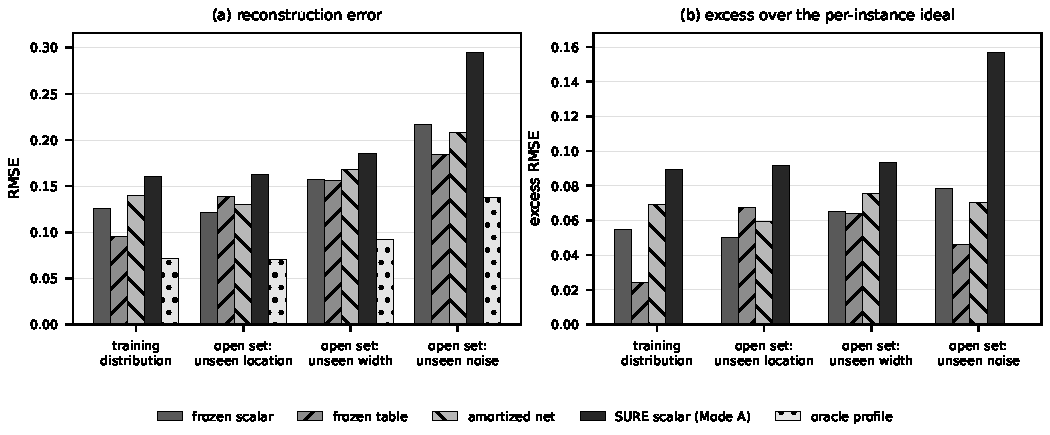
\includegraphics[width=\linewidth]{figures/probe.pdf}
\caption{A minimal probe of the risk gap on a constructed open inversion task (\texttt{experiments/probe.py}). Panel (a): each rule's reconstruction error; panel (b): excess over the per-position ideal. The corpus-fitted table is best on the training distribution and the only rule within a third of the ideal, its excess growing by $1.9$ to $2.8$ on the open set while the ideal is unchanged; per-instance SURE, the analytic path's rule and the amortized map do not close the headroom (the cost side, Section~\ref{sec:cost}).}
\label{fig:probe}
\end{figure}

\subsection{Relation to Uncertainty Quantification}

Predictive uncertainty splits into data uncertainty (observation noise) and epistemic uncertainty (ignorance of model parameters, shrinking with training data) \citep{kendall2017}. The latter statistically represents Mode~B's source of values --- parameters uncertain because a finite corpus determines them, resampling giving different values --- while Mode~A rules have no such freedom. It calibrates well on closed benchmarks, but these remain in-distribution, leaving no distribution to calibrate against on the open set.

\subsection{Clues to Endogenous Mechanisms}

Mode~A has long-standing neuroscience counterparts: predictive coding treats visual cortex as higher levels predicting the input to lower ones, which return only prediction errors \citep{rao1999}, and the free-energy principle describes perception as inversion of a generative model \citep{friston2009,friston2010} (tutorials \citep{bogacz2017}). Their common form is exactly Paradigm I: context rules endogenous to one generative objective, prediction values computed online from current evidence, not looked up from a frozen table. The paper does not claim these can be copied into engineering, only that the evolution-selected architecture falls on the Mode~A side of the decision axis, consistent with the negation conclusion.

\subsection{Existence and Cost of Mode A}
\label{sec:cost}

Two paths substantiate existence: the analytic-invariant path (calibrated intrinsics, geometric computations, coupling strengths solved online from current observations, their values given by evidence and calibration, bypassing the corpus) and the per-instance optimization path (test-time optimization and online inversion solving rule values per input \citep{sun2020}, transductive learning its near-distribution precedent \citep{vapnik1995}); predictive coding is a third clue. Within A0's range Mode~A is therefore not empty, so fixed-memory alone cannot be complete while a combination with Mode~A can; where A0 fails no mechanism is complete, though Mode~B fails there too.

The analytic-invariant path costs constant-to-linear, negligible; the per-instance optimization path about $10^2$ to $10^3$ forward computations; iterative inference lies between, by iteration count. Mode~B's temptation comes exactly from this difference --- one optimization replaced by one forward pass --- as does the composite-system motivation: Mode~B in cost-sensitive, in-distribution stages, Mode~A in the critical rule-generation stage.

\subsection{Correspondence with Adaptive Control and Online Optimization}

Gain-scheduled control requires measurable, exogenous scheduling variables and looks up or computes controller parameters from the operating condition --- exactly ``rule values instantiated by current evidence'' \citep{shamma1990} --- while auto-tuning and model-reference adaptive control generate the control law online \citep{astrom1995}. Conversely, an offline-tuned fixed gain table embodies Mode~B, and gain scheduling by a fixed schedule table is the control-theoretic ``move one level up'' of the reach section, the schedule table still given by offline experience. Online convex optimization likewise belongs to Mode~A \citep{hazan2016}; control-law online tuning has Lyapunov guarantees that Mode~A inference lacks, an analogous theory being its main engineering gap.

\subsection{Abstention and the Composite Path}

Detect-and-abstain is accurate in-distribution, detecting and refusing on out-of-distribution anomalies. But completeness requires correct answers on all inputs, and an abstaining system faces the same decision axis on the inputs it does not refuse; if the refusal rule is fixed-parameterized, detection fails on the open set too --- the known difficulties of out-of-distribution detection \citep{hendrycks2016}. Abstention therefore does not escape the axis, only moving failure from answering to detection; nor is it a dead end, since an evidence-instantiated refusal criterion permits fallback to a measurement-model-guided search, confining failure to detection.

Composite systems combine fixed-memory proposal of candidates and likelihoods with Mode~A rule generation and near-tree arbitration. The credit for completeness goes to the Mode~A mechanism, while the Mode~B components still earn their keep, consistent with the weak claim's delimitation; existing end-to-end systems thus remain legitimate in-distribution, only the Mode~A loop of rule generation needing to be added. Online reconstruction exhibits the granularity: SurfelNeRF updates a learned scene representation by per-scene optimization, splitting into a corpus-fitted geometry-and-appearance component and an inference-time consistency solve \citep{gao2023surfelnerf} --- Mode~B and Mode~A respectively.

\subsection{Design Implications}

Three engineering questions follow: where the rule's values come from (corpus statistics, manual setting, current evidence, analytic calibration); whether they are frozen at inference (frozen Mode~B, online instantiation Mode~A); and who on the open set instantiates the rule (no responsible mechanism, no completeness for open inversion tasks) --- mapping respectively onto the operational readings of Definition~3, Proposition 4 and Theorem 5, with the reverse direction, deciding an existing implementation's mode, the procedure of Section~\ref{sec:procedure}. The minimal legitimate composite form is as above.

\subsection{Limitations}

Four limitations. First, Criterion P4's satisfiability is load-bearing: Section~\ref{sec:p4} gives its two components --- demand exactly identifiable from a fixed corpus fails the barrier condition, rare fine-scale demand reversals fail the realization condition --- both outside the class, where a fixed-memory component can be complete (Example~\ref{ex:p4fails} the first boundary). No magnitude claim: the barrier-to-gap proposition yields only the task-attached constant $\kappa$ of \eqref{eq:floor}, not an unbounded gap. The positive claims additionally need Assumption~A0: tasks whose demand depends on unobserved structure with no evidence trace fail it, leaving no complete mechanism. Second, the falsification targets ``solo use is complete''; for composites it gives only necessary-condition-level guidance --- a fixed-memory component in a combination still has Mode~B rules, completeness requiring another Mode~A mechanism --- not sufficient conditions. Third, machine verification covers the carrier-independent algebraic core and structured general forms; the rest are the three items of Section~\ref{ch:verify}. Fourth, Mode~A's implementation has existence paths and cost magnitudes but no construction scheme. Empirical quantification remains future work (the probe of Section~\ref{sec:probe}, a first measurement): rule-family comparisons on a benchmark such as \citep{leuschner2021} against data-consistent frozen baselines, and estimation of a task's barrier separation and realization level --- no experimental commitment about a real deployment's open set.

%%%%%%%%%%%%%%%%%%%%%%%%%%%%%%%%%%%%%%%%%%%%%%%%%%%%%%%%%%%%%%%%%%%%%%
%% --- inlined from sections/08-conclusion.tex
%%%%%%%%%%%%%%%%%%%%%%%%%%%%%%%%%%%%%%%%%%%%%%%%%%%%%%%%%%%%%%%%%%%%%%
\section{Conclusion}
\label{ch:conclusion}

Once context-rule values are solidified by a corpus and frozen at inference, no fixed-memory component is complete for open inversion tasks on its own. The decision axis: ill-posedness forces context; Lemma 1 excludes the global scalar, and Lemma 2 frozen extrinsic coefficients, from realizing a heterogeneous profile, converging the criterion onto the source; Criterion P4 and Lemma 3 require evidence-instantiated values; Proposition 4 completes the classification; Theorem 5 closes. Equivalently, no frozen rule family is uniformly optimal on the open set, offering at most in-distribution guarantees or guarantees vetted by analytic data consistency, since pointwise or expected worst-case guarantees require evidence instantiation. The amortization gap records the empirical Mode B gap, No-Free-Lunch the algorithm-level universal negation; between them this paper supplies the component-level completeness negation, a unified decision axis, and, against No-Free-Lunch, its converse on open inversion tasks.

Beyond neural networks the reach holds: Markov random fields, conditional random fields, Gaussian mixture models, dictionary learning, kernel methods and others whose context rules are carried by offline-trained or hand-set parameters are Mode B, within the same falsification; random fields with coupling strengths computed online from current evidence are Mode A, outside the negation. The boundary: tasks whose demand is exactly identifiable from a fixed corpus are outside the class, where a fixed-memory component can be complete; the falsification stops where the demand becomes freezable. The exclusion is independent of the quadratic smoothing form: Lemma 1 holds for a separable data term, any even differentiable pairwise potential and no convexity; its minimal obstruction is an equivalence, not a sufficient condition---one position whose required strength ratio changes between two admissible configurations. This excludes every frozen coefficient family, however large; the global scalar, requiring the ratio to be common to all positions, is the shallowest member of the excluded class, not a special case defended separately.

Negation is not disparagement: their closed-benchmark achievements are genuine; only the universal claim ``solo use is complete'' is negated, not their usefulness in combinations, and Mode A's engineering implementation, the decision axis's other side, is left to future work.


% JMLR requires an Acknowledgements and Disclosure of Funding section,
% placed before the appendices and the references. It must declare both
% (i) financial activities supporting the work and (ii) competing
% interests outside the submitted work.
%
% The author has confirmed that this work received no specific funding,
% so the funding declaration below is final (no placeholder remains).
\acks{The Lean~4 development reported in Section~\ref{ch:verify} was carried out with the Lean~4 proof assistant and its mathematical library Mathlib; the author thanks the Mathlib community for maintaining it. The verified artifact described in Section~\ref{ch:verify} is distributed in the \texttt{lean-proof} directory of the paper's repository, together with the \texttt{lean-toolchain} file that pins the toolchain version.

Funding: this research received no specific funding.

Competing interests: the author declares no competing interests.}

\vskip 0.2in
\bibliography{reference}

% The artifact index (layout, reproduction, axiom budget, the map from paper
% items to Lean declarations, and the premise lists of the load-bearing
% declarations) is published as the separately hosted online appendix, built
% from online-appendix/ by  ./build.sh appendix . It is deliberately kept out
% of this file: appendix pages count toward the JMLR page limit, and the paper
% points to the online appendix from its verification section instead.

\end{document}
